%\def\mytitle{060112\_Dissertation}
%\def\myauthor{Andrew Beck}
%\input{../Beck_disstemplate_MASTER}

\chapter{Comparison of the Live-Attenuated Japanese Encephalitis Vaccine SA14-14-2 to Its Virulent Parental Strain SA14 By Deep Sequencing}

\section{Abstract}
\Gls{je} is a mosquito-borne flavivirus disease that is controlled by vaccination. Live attenuated \gls{jev} vaccine strain SA14-14-2 was derived by serial passage of \gls{wt} strain SA14 in hamster kidney, licensed in China in 1989 and 8 other countries thereafter. It has been used as a component of childhood immunization programs throughout Asia with approximately 400 million doses distributed.  Although the vaccine is considered highly safe and effective, and some progress has been made to elucidate the discrete mechanisms of attenuation, the complexity of the attenuating passage history for SA14-14-2 has prevented full resolution of the genotype for the vaccines. We have previously investigated another live attenuated flavivirus vaccine, yellow fever strain 17D, by deep sequencing and shown that the \gls{wt} parent Asibi has a typical quasispecies structure of a \gls{rna} virus while 17D has a homogeneous structure suggesting that attenuation is in part due to lack of diversity of the 17D genome. Using a similar deep sequencing approach, the subpopulation structures of two examples of SA14-14-2 vaccine were compared to those of the \gls{wt} parental strain SA14. SA14-14-2 virus was found to have lower diversity than the parental strain; this pattern is highly localized, along with limited observation of \gls{wt} sequence content in the viral subpopulation. The findings demonstrate that similar lack of diversity for two live attenuated flavivirus vaccines may indicate a characteristic of live-attenuated RNA viruses generally. These observations indicate that diversity of live viral vaccines should be considered in assessments of vaccine safety and quality.


\section{Introduction}
\Gls{jev} is the etiologic agent of \gls{je}, which is a major threat to public health across a range comprising 24 countries in east and southeast Asia. \Gls{jev} is a member of the family \emph{Flaviviridae}, genus \emph{flavivirus}, and has a ~50\gls{nm} enveloped particle, containing a single-stranded, positive-sense \gls{rna} genome of 11\gls{kb}, which encodes 3 structural genes (\gls{c}, \gls{prm}, \gls{e}) and 7 nonstructural genes (\gls{ns}1, \gls{ns}2A, \gls{ns}2B, \gls{ns}3, \gls{ns}4A, \gls{ns}4B, \gls{ns}5). The polyprotein sequence is flanked by 5’ and 3’ \glspl{utr}. \Gls{jev} is the prototype member of a same-named serogroup that includes a number of arthropod-borne pathogens causing infection of the central nervous system in humans, including \index{Viruses, Miscellaneous!\Acrfull{wnv}}\gls{wnv}, \index{Viruses, Miscellaneous!\Acrfull{mvev}}\gls{mvev}, \index{Viruses, Miscellaneous!\Acrfull{usv}}\gls{usv}, and others. The ecology of \gls{jev} transmission is complex, in which the virus is principally vectored by mosquitoes of the genus \emph{Culex}, in particular \emph{Cx. tritaeniorhynchus}, which is ubiquitously found across the range of the virus and associated with human cases \parencite{Miller:2012bx}. Amplification hosts include domestic pigs and wading birds; humans are considered dead-end hosts, encountering the virus niche by proximity to rice cultivation or swine husbandry \parencite{Zhao:2014kb}. 

Annual case burden is estimated to be 68,000 in total across the endemic and epidemic ranges, mostly in children, despite widespread access to vaccination \parencite{Campbell:2011gv}.
Although the pathogenesis of \gls{je} disease is poorly understood, the virus is observed histologically to invade the mammalian central nervous system, a finding observed in multiple animal models of \gls{jev} infection \parencite{Li:2015cf,Myint:2014dj,WorldHealthOrganization:2003tq}. In severe cases, \gls{jev} infection may cause permanent neurological sequelae, including paralysis, weakness, or impaired cognition \parencite{Yin:2015fi}. Owing to the geographic ubiquity of \gls{jev} in Asia, severity of \gls{je} disease, and economic impacts of long-term care, a series of vaccines has been developed, beginning with formalin-inactivated mouse brain preparations using the Nakayama-NIH or Beijing-1 strain in the 1950s and subsequently replaced by formalin-inactivated cell-culture derived vaccines. The live-attenuated vaccine strain SA14-14-2, produced since 1988 by the Chengdu Institute of Biological Products in China, was the only live-attenuated \gls{jev} vaccine using the entire \gls{jev} genome.
SA14, the parental \gls{wt} strain of SA14-14-2, was prepared from a pool of \emph{Cx pipiens} mosquitoes in Xi’an, China. The resulting preparation was passaged 100 times in \gls{phk} cells, then in a complex series of mammalian tissues, from which plaque picks were periodically taken. 

The full passage history of SA14-14-2 is shown in Figure \ref{JEV_tree}, with reference to other live-attenuated \gls{jev} vaccine strains studied or developed along other points on the same passage series.  The vaccine is greatly attenuated with respect to both direct mouse neurovirulence and neuroinvasion (entry to the central nervous tissues from periphery) to the extent that intracerebral inoculation of one million \gls{pfu} causes no clinical or histopathologic signs of infection in mice and monkeys \parencite{WorldHealthOrganization:2014wca}. 
\Gls{rna} viruses encode a \gls{rna}-dependent-\gls{rna} polymerase, which unlike \gls{dna} polymerases lacks proof-reading activity and, consequently, \gls{rna} virus genomes exist as a quasispecies of related \gls{rna} sequences. Varying levels of naturally-occurring subpopulation diversity arises during the lifecycle of  \gls{rna} viruses, a consequence of large population sizes and error-prone replication. In the case of empirically-derived vaccine strains such as SA14-14-2, the population structure of the virus is likely to carry informative signals of passage history, providing an association of specific elements of viral diversity with the controlled vaccine phenotype. Current \gls{who} technical specifications for live-attenuated \gls{jev} vaccines does not prescribe a standard genotype, owing to a multiplicity of reported genotypes for the vaccine, and the acceptable safety margins afforded by empiric, \emph{in vivo} qualification of the vaccine \parencite{Ni:1995vy, Nitayaphan:1990vr, Song:2012iw, Aihara:1991tn, WorldHealthOrganization:2014wca}. In the case of arthropod-borne viruses such as \gls{jev}, changes in population structure in the empiric transition to vaccine phenotype are likely to be especially meaningful, owing to the complex multiple-host niches occupied by the virus in nature to derive a live vaccine strain that is attenuated in mammalian hosts and not mosquito competent. In this paradigm, the properties of the viral “quasispecies” population may effect pathogenesis or conversely attenuation; low-abundance populations in a virus may exert wild type effects or otherwise determine the course of pathogenesis \parencite{Vignuzzi:2006ju}. In a strict sense, this model of the virus lifecycle predicts that some level of population diversity is necessary to traverse infection barriers or host tissues. Because the infection caused by the \gls{jev} vaccine is attenuated both for neurotropic disease and characterized by low viremia, a reasonable hypothesis arises that SA14-14-2 is of lower diversity than the \gls{wt} strain from which it was derived.

\Gls{ngs} studies represent a family of \emph{in silico} techniques with potential to assess and predict phenotype of vaccines, particularly by the resolution of population substructure and detection of contaminants \parencite{Prachi:2013hm, Luciani:2012em, Victoria:2010kf}. Previous work on this topic using \gls{ngs} techniques has observed that the related flaviviral live-attenuated \gls{yfv} vaccine strain 17D is of lower diversity than the \gls{wt} parental Asibi strain from which the vaccine was derived \parencite{Beck:2014cm}. Like SA14-14-2, 17D was passaged to attenuate in a series of multiple, alternating tissues, leading to the occurrence of viral population bottlenecks or purifying selection for the vaccine genotype \parencite{Theiler:1937wy}. Because SA14-14-2 represents a closely related live attenuated vaccine to \gls{yfv}, \gls{jev} offers a unique opportunity to confirm that patterns of low diversity are a feature of live-attenuated strains, and to contribute to a framework by which this information is used to guide expectations of live vaccine safety and stability.



\section{Results}
\subsection{Read Coverages}
Mean read coverage of the \gls{wt} strain SA14 was 2262.337 (median=2188, \gls{sd}=702.368). Mean read coverage of the vaccine strain SA14-14-2/P1 was 2258.343 (median=2299, \gls{sd}=501.016). Mean read coverage of the vaccine strain SA14-14-2/P2 was 2263.687 (median=2028, \gls{sd}=1020.042) [Figure \ref{JEV_coverage}].

\subsection{Consensus Sequences}
\subsubsection{Comparison of Newly Sequenced SA14 to Previously Reported SA14 Sequences}
Three other strains of SA14 have been previously sequenced at the consensus level, and were compared in reference to the newly sequenced SA14 strain by consensus [Table \ref{JEV_SA14_consensus}]. Genbank accession M55506 \parencite{Nitayaphan:1990vr} differed from SA14 at 11 amino acids (\gls{e}-E244G, \gls{e}-A315V, \gls{e}-K439R, \gls{ns}1-G292S, \gls{ns}1-R339M, \gls{ns}2A-N2K, \gls{ns}2A-A40V, \gls{ns}2A-V106I, \gls{ns}3-K73R, \gls{ns}5-K328E, \gls{ns}5-N644T). Genbank accession D90194 \parencite{Aihara:1991tn} differed from SA14 at five amino acids (\gls{e}-E244G, \gls{e}-P334S, \gls{ns}3-K73R, \gls{ns}3-A235V, \gls{ns}5-G741D). Genbank accession JEU14163 \parencite{Ni:1994vs} differed from SA14 at four amino acids (\gls{ns}1-G292S, \gls{ns}2B-M102T, \gls{ns}3-K73R, \gls{ns}4A-K79R). Only one of the 16 amino acid substitutions (\gls{ns}3-K73R) was conserved between all of the previously reported strains, in reference to SA14.
\subsubsection{Comparison of SA14 to SA14-14-2/P1 and SA14-14-2/P2}
In comparison to the newly sequenced parental \gls{wt} strain SA14, SA14-14-2/P1 and SA14-14-2/P2 were identical to each other, each containing 53 nucleotide differences, of which 22 were amino acid substitutions [Table \ref{JEV_main_consensus}]. With respect to viral genes, one amino acid substitution was observed in \gls{c} (\gls{c}-L66S), eight \gls{e} (\gls{e}-L107F, E138K, I176V, T177A, E244G, Q264H, A315V, K439R), three in \gls{ns}1 (\gls{ns}1-G292S, R339M, D351H), two in \gls{ns}2A (\gls{ns}2A-N2K, A40V), two in \gls{ns}2B (\gls{ns}2B-E63D, N65G), three in \gls{ns}3 (\gls{ns}3-M59V, A105G, A235V), one in \gls{ns}4B (\gls{ns}4B-I106V), and three in \gls{ns}5 (\gls{ns}5-H386T, Q639H, V671A).
\subsection{Diversity and Genetic Distance of Vaccines, Relative to the Wild-Type Strain}
\subsubsection{Summary of Diversity for Entire Strain Genomes and For Gene Segments}
Diversity was estimated at individual nucleotide positions across the genomes of SA14, SA14-14-2/P1, and SA14-14-2/P2 [Figure \ref{JEV_entropy_whole}]. For all nucleotide positions in entire open reading frames (n=10296), mean normalized entropy for the \gls{wt} strain SA14 was 0.103 (median=0.100, \gls{sd}=0.049). Mean normalized entropy for the vaccine strain SA14-14-2/P1 was 0.103 (median=0.100, \gls{sd}=0.051). Mean normalized entropy for the vaccine strain SA14-14-2/P2 was 0.100 (median=0.094, \gls{sd}=0.057). Sets differed significantly by the Kruskal-Wallis rank-sum test (X$^2$= 24681.59, \gls{df}=2, p<0.001). Between the strains, the rank-order of estimated diversity for each gene segment was variable [Table \ref{JEV_entropy_genewise}].
\subsubsection{Summary of Diversity for Proposed SA14-14-2 Genotype}
When considering the set of nucleotide positions containing the consensus amino acid substitutions between SA14 and SA14-14-2 strains only (n=22), mean normalized entropy for the \gls{wt} strain SA14 was 0.121 (median=0.093, \gls{sd}=0.099). Mean normalized entropy for the vaccine strain SA14-14-2/P1 was 0.097 (median=0.097, \gls{sd}=0.043). Mean normalized entropy for the vaccine strain SA14-14-2/P2 was 0.095 (median=0.090, \gls{sd}=0.049). Strains differed significantly by the Kruskal-Wallis rank-sum test (X$^2$=56.524, \gls{df}=2,  p < 0.001).
\subsubsection{Individual Diversity of Amino Acid Substitution Sites for Proposed SA14-14-2 Genotype}
When considering the set of nucleotide positions containing the consensus amino acid substitutions between SA14 and SA14-14-2 strains only, differences in summarized diversity were unequally localized between discrete genes [Table \ref{JEV_entropy_sites_summary}].  Genes containing 14 of the 22  sites were demonstrated to have greatest relative normalized entropy compared to the vaccine strains; mean values for these genes were as follows: \Gls{e}:(n=8 SA14=0.169, SA14-14-2/P1=0.090, SA14-14-2/P2=0.092), \gls{ns}2A:(n=2, SA14=0.143, SA14-14-2/P1=0.101, SA14-14-2/P2=0.111) \gls{ns}3:(n=3, SA14=0.106,  SA14-14-2/P1=0.093, SA14-14-2/P2=0.093), and \gls{ns}4B:(n=1, SA14=0.080, SA14-14-2/P1=0.032, SA14-14-2/P2=0.051).

Differences in mean entropy were further localized to a subset of positions within the 14 sites identified to have high relative diversity in SA14 [Table \ref{JEV_entropy_individual}, Figure \ref{JEV_barplot}]. These positions were, respectively, 1296-\gls{e}-L102F:(SA14=0.137, SA14-14-2/P1=0.097, SA14-14-2/P2=0.110), 1506-\gls{e}-T177A:(SA14=0.175, SA14-14-2/P1=0.084, SA14-14-2/P2=0.140), 1708-\gls{e}-E244G:(SA14=0.489, SA14-14-2/P1=0.081, SA14-14-2/P2=0.108), 1921-\gls{e}-A315V:(SA14=0.112, SA14-14-2/P1=0.076, SA14-14-2/P2=0.083), 2293-\gls{e}-K439R:(SA14=0.193 SA14-14-2/P1=0.037, SA14-14-2/P2=0.062), 3652-\gls{ns}2A-A40V:(SA14=0.222, SA14-14-2/P1=0.127, SA14-14-2/P2=0.175), and 4782-\gls{ns}3-M59V:(SA14=0.195, SA14-14-2/P1=0.142, SA14-14-2/P2=0.160). Genetic distance (\gls{rmsd}) of these sites in the vaccine strains relative to SA14 was computed using the nucleotide frequencies in the alignments, and revealed a pattern of stable selection for the vaccine genotype [Figure \ref{JEV_scatter_RMSD}].

\subsection{Variant and Wild-Type Revertant Structure of SA14-14-2 Strains}
For the \gls{wt} strain SA14, 62 \glspl{snv} were observed in total; of these, 35 were coding changes relative to the consensus sequence. For the vaccine strain SA14-14-2/P1, 92 \glspl{snv} were observed in total; of these, 44 were coding relative to the consensus. For the vaccine strain SA14-14-2/P2, 72 \glspl{snv} were observed in total; of these, 35 were coding relative to the consensus [Figure \ref{JEV_vphaser}]. Variants were consistently observed between SA14-14-2/P1 and SA14-14-2/P2; of the 121 possible unique \glspl{snv} observed between either of the two vaccine strains, 43 (35.5\%) were common. 20 of the 43 variants were observed that coded for amino acid substitutions with respect to the [identical] consensus sequences of the vaccines [Table \ref{JEV_variants_concordant}]. Two \gls{wt} revertant amino acids were observed in common between the vaccines, \gls{ns}1-V392G (0.9572\% in P1, 1.365\% in P2) and \gls{ns}3-V235A (1.693\% in P1, 1.707\% in P2).
\subsection{Selection Analysis and $dN/dS$ Ratios}
Over the open reading frame of each strain, $dN/dS$ for SA14 was 0.413, for SA14-14-2/P1 was 0.474, and for SA14-14-2/P2 was 0.419. When considering individual genes, $dN/dS$ ratios were not equal between genes for both the \gls{wt} and vaccine strains [Table \ref{JEV_genesegment}]. Broadly,$dN/dS$ ratios for all strains did not exceed 1.000, indicative of negative or purifying selection. Of the segments with $dN/dS$ ratios equal to or greater than 1, indicating neutral or positive selection, two were observed in the SA14 alignment (prM=1.073, \gls{ns}1=1.246), two were observed in SA14-14-2/P1 (E=1.023, \gls{ns}4B=1.710), and one was observed in SA14-14-2/P2 (\gls{ns}4B=1.871). 
When analyzed using a 20-codon sliding window, regions of the \gls{jev} genome were observed to have values greater than 1.000, [Table \ref{JEV_high20_dnds}, Figure \ref{JEV_20codon}] indicating the possibility that these particular domains are less conserved in the genotype or are under positive selection. In SA14, windows of high-ranking $dN/dS$ were clustered in \gls{e}, \gls{ns}1, and \gls{ns}3. In both SA14-14-2 strains, high-ranking $dN/dS$ values were clustered in the \gls{e} gene.
\section{Discussion}
\subsection{Resolution of Consensus for SA14 and SA14-14-2 Strains Using Limited Sequence Information}
Resolution of the genotypes of SA14 and S14-14-2 are complicated by both a lack of publicly available sequences and dissimilarity of passage history for those reported strains. When comparing the SA14 strain sequenced in this study to those publicly available, very limited divergence was observed between SA14 and the two most recently sequenced strains of SA14: Genbank accession D90194 (5 amino acid differences) \parencite{Aihara:1991tn} and Genbank accession JEU14163 (4 amino acid differences) [Table \ref{JEV_SA14_consensus}]. Greater divergence was observed in reference to Genbank accession M55506 (11 amino acid differences) \parencite{Nitayaphan:1990vr}. Because the SA14 sequence used in this study was a single passage from a low-passage institutional collection stock, it is likely to closely represent the originating SA14 genotype, and therefore is an appropriate reference by which to infer the genotype of SA14-14-2 vaccine strains.
SA14-14-2/P1 and SA14-14-2/P2 differ by a single passage in Vero cells, and were identical in reference to the SA14 [Table \ref{JEV_main_consensus}]. The observed substitutions confirmed, with limited exceptions, the genotype of the vaccine as reported by Gromowski et. al., in which a infectious clone of SA14-14-2 was constructed and used to investigate vaccine determinants of mouse neurovirulence, however, the SA14-14-2 genotype reported in this study does not contain substitutions in either untranslated region of the virus genome as previously reported in reference to a recombinant infectious clone of \gls{wt} strain India/78 \parencite{Gromowski:2015cg,Gromowski:2015et}. Additionally, the amino acid substitutions \gls{e}-E244G, \gls{e}-A315V, \gls{e}-K439R, \gls{ns}1-G292S, \gls{ns}1-R339M, \gls{ns}1-D351H, \gls{ns}2A-N2K, \gls{ns}2A-A40V and \gls{ns}5-Q639H, conserved across SA14-14-2 strains and were not previously hypothesized to represent the vaccine genotype. Because these substitutions were observed relative to a low-passage stock of the parent SA14, it is plausible that the substitutions represent a more accurate SA14-14-2 genotype than previously investigated.

\subsection{Previous Investigations of Neurovirulence Determinants}
Neurovirulence studies on discrete genomic determinants of SA14-14-2 attenuation have been investigated by infectious clone systems, although very limited work of this type has been reported. In an experiment to investigate the stability of the vaccine, SA14-14-2 was passaged 11 times in suckling mouse brain, and this increased the neurovirulence phenotype of the strain for mice \parencite{Yang:2014io}. In the same study, Yang et al. observed by plaque picking and conventional Sanger sequencing a set of intermediate, quasi-genotypes that were selected during in mouse brain passage, including the \gls{wt} revertants \gls{e}-F107L, \gls{e}-K138E, \gls{e}-G244E \parencite{Yang:2014io}. Construction of an infectious clone of \gls{wt} \gls{jev} strain JaOArS982 was reported by Sumiyoshi et. al, in which the envelope substitution \gls{e}-F107L was observed to reduce mouse neurovirulence \parencite{Sumiyoshi:1992vf,Sumiyoshi:1995fl}. Residues \gls{e}-107L and \gls{e}-138E were also observed by Gromowski et al. to be potential determinants of attenuation for mouse neurovirulence in a study using a \gls{jev} infectious clone system to study each whole-gene set of vaccine substitutions \emph{en masse}, although in this study the substitutions were not assayed individually \parencite{Gromowski:2015et}. Significantly, this study reported that the entire envelope genotype was sufficient to attenuate the mouse neurovirulence phenotype for the vaccine.
\subsection{Features of Stability and Low Diversity for SA14-14-2 Vaccine Strains}
\emph{In silico} techniques were previously used to compare the \gls{yfv} \gls{wt} Asibi strain with live-attenuated vaccine strain 17D [Chapter 3]. These studies showed that \gls{wt} Asibi had a typical quasispecies structure of a \gls{rna} virus while 17D vaccine had a relatively homogeneous population and it was hypothesized that the lack of diversity contributes to the attenuated phenotype of the 17D vaccine \parencite{Beck:2014cm}. This paradigm for live attenuated \gls{rna} viruses was hypothesized to be conserved for serially-passaged viral vaccines, specifically \gls{wt} \gls{jev} strain SA14 and its live attenuated vaccine derivative SA14-14-2. Although live attenuated SA14-14-2 has been found to be both effective and safe, derivation of the vaccine utilized a complex passage process in multiple cell types and hosts. SA14-14-2 was derived from SA14-5-3, a strain that was attenuated but not sufficiently immunogenic in clinical trials [Figure \ref{JEV_tree}]. SA14-5-3 was passaged five times in mouse skin, and plaque-picked to generate SA14-14-2; the short adapting passage series produced a strain with increased immunogenicity and seroconversion rates in children \parencite{Huang:1982jd}. 

It was hypothesized that the complex selection pressures exerted upon the vaccine by serial passage would be resolvable in the population structure of the vaccine. These hypotheses were confirmed for the \gls{jev} strains considered in the study, however diversity effects were highly localized. Low diversity was a general feature of the vaccine strains in comparison to SA14. When restricting the analysis to discrete genes, the effect was most apparent for gene segments in which putative attenuating mutations are clustered, and as such was especially apparent in the envelope protein gene. As expected, loss of diversity is most apparent for the 22 sites shown to carry amino acid substitutions that distinguish SA14 from SA14-14-2. Notably, a restricted set of these sites were observed in which loss of diversity for the vaccine is especially great; in this set are included \gls{e}-F107L and \gls{e}-G244E that were previously observed to revert under passage in mouse brain at the population level. A later infectious clone study demonstrated that substitution \gls{e}-G244E (relative to SA14-14-2) conferred a lethal neurovirulence phenotype in mice for infectious clone derived SA14-14-2 strains carrying the \gls{wt} glutamic acid residue \parencite{Yun:2014jr}. Also notably, both the coding variant populations [Table \ref{JEV_variants_concordant}] and the diversity profiles [Tables \ref{JEV_entropy_genewise}, \ref{JEV_entropy_sites_summary}, \ref{JEV_entropy_individual}] were similar between SA14-14-2/P1 and SA14-14-2/P2, indicating negligible fluctuation in population frequencies between the two vaccine strains on single Vero cell passage [Figure \ref{JEV_tree}]. These findings are consistent with those of Yang et al., in which Vero passage did not appear to perturb the phenotype of the vaccine \parencite{Yang:2014io}. 

\subsection{Patterns of Selective Pressure Are Typical For Arboviruses}
The findings are consistent with previous comparison of population structure for \gls{yfv} strains Asibi and 17D-204 \parencite{Beck:2014cm}. Similarly by consensus, the attenuation of 17D produced a vaccine genotype with a number of amino acid substitutions in the envelope gene (8 of 20 substitutions [Table \ref{WHO_standard_YFV}]), although the attenuation of \gls{yfv} is presumed to be influenced by both structural effects in the envelope as well as a phenomenon of \gls{ifn} antagonism; this has been proposed based on functional studies of both the \gls{yfv} \gls{ns}4B gene and envelope residues \parencite{Lee:2008gd}. By population, diversity in the \gls{yfv} genome is also localized to the envelope protein in the same proportion as in \gls{jev}, with 3 of 9 major coding variants present reported in the Asibi genome [Chapter 3, Table \ref{JEV_high20_dnds}]. The direct comparison of population structure change for \gls{yfv} and \gls{jev} vaccines is however complicated by the different \gls{wt} manifestations of \gls{yf} (viscerotropism) and \gls{je} disease (neurotropism), and as well the different ecological niches in which the viruses are encountered in nature. Selection pressures along SA14 and SA14-14-2 genomes were broadly observed to be negative ($dN/dS$<1), which is an expected result for arboviruses, and is presumably due to the complex trade-offs in fitness required for the virus to productively infect multiple \gls{wt} hosts. 

However counter-intuitively, some regions were observed to be influenced by positive selection ($dN/dS$>1); for the vaccines, this was localized to the envelope and \gls{ns}4B genes [Table \ref{JEV_high20_dnds}]. It is possible that the signal of selection at these regions shows localization of particular instability for the vaccine genotype under cell culture, however the stability of SA14-14-2 under Vero cell passage has been attested experimentally \parencite{Yang:2014io}. Also counter-intuitively, some genes in the vaccine strains were of greater diversity in the vaccine strains than in SA14, however, for amino acid substitutions known to influence the phenotype of SA14-14-2, loss of diversity in the vaccines was readily apparent. 

The significance of these persistent subpopulations to the phenotype of the vaccine, if any, is not known. However, cases in which low-frequency viral populations are associated with phenotype in a continuous manner have been studied. A nonclinical characterization \gls{yfv} 17DD substrain vaccine was performed after adapting the seed virus to \glspl{cef} (17D vaccines are produced in embryonated eggs). The resulting vaccine, when tested using a standard monkey neurovirulence assay, was of greater neurovirulence in monkeys by histological assessment, however, this was not statistically significant \parencite{Freire:2005iw}. The consensus sequences were identical, suggestive of a population-level effect.


\section{Conclusions}
Previous studies comparing the population structures of another live-attenuated viral vaccine, \gls{yfv} 17D, revealed that fluctuations in viral subpopulations frequently accompany the complex selection pressures encountered in attenuation by serial passage. It is especially significant that the present findings on \gls{jev} are in agreement with clonal sequencing studies of SA14-14-2 that were previously reported. Considerable support is presented in these findings to suggest that changes in phenotype for SA14-14-2 vaccines may be predicted based on features of the viral quasispecies, which in this case were repeatably observed between two vaccine strains. Patterns of diversity chance in transition to the SA14-14-2 genotype are localized to regions of the genome previously shown to influence the attenuation of neurovirulence for the vaccine in infectious clone studies. Accordingly, the presented data represents a confirmation of previously observed patterns for \gls{yfv}, and establishes a framework by which to construct further studies on the pathogenic significance of flaviviral vaccine subpopulations.




\clearpage
% Table with SA14 comparison.
\begin{table}[h]
	\centering
	\begin{ThreePartTable}
		\caption{Amino acid substitutions differentiating the SA14 strain sequenced in this study to 
			that of three others previously reported.}
		\taburowcolors [2]1{gray!20 .. white}
		% This is the filler table for checking formats.
% Please add the following required packages to your document preamble:
% \usepackage{booktabs}
% \usepackage[table,xcdraw]{xcolor}
% If you use beamer only pass "xcolor=table" option, i.e. \documentclass[xcolor=table]{beamer}
\begin{tabu}{X[1.2,l]X[.75,l]X[.75,l]X[.75,l]X[l]X[l]X[1.1,l]}
	\rowfont[1]{\bfseries}
\toprule
Nucleotide Position & Gene & Codon & SA14\tnote{a} & M55506\tnote{b} & D90194\tnote{c} & JEU14163\tnote{d} \\ \midrule
1708 & E    & 244 & E & G & G & - \\
1921 &     & 315 & A & V & - & - \\
1977 &     & 334 & P & - & S & - \\
2293 &     & 439 & K & R & - & - \\
3351 & NS1  & 292 & G & S & - & S \\
3493 &   & 339 & R & M & - & - \\
3539 & NS2A & 2   & N & K & - & - \\
3652 &  & 40  & A & V & - & - \\
3849 &  & 106 & V & I & - & - \\
4519 & NS2B & 102 & M & - & - & T \\
4825 & NS3  & 73  & K & R & R & R \\
5311 &   & 235 & A & - & V & - \\
6700 & NS4A & 79  & K & - & - & R \\
8658 & NS5  & 328 & K & E & - & - \\
9607 &   & 644 & N & T & - & - \\
9898 &   & 741 & G & - & D & - \\ \bottomrule
\end{tabu}
		\begin{tablenotes}
			\item[a] Sequenced in this study.
			\item[b] \parencite{Nitayaphan:1990vr}
			\item[c] \parencite{Aihara:1991tn}
			\item[d] \parencite{Ni:1994vs}		
		\end{tablenotes}
	\label{JEV_SA14_consensus}
	\end{ThreePartTable}
\end{table}

\clearpage
% Table with SA14/SA14-14-2 comparisons.
%\begin{table}[h]
%	\centering
	\begin{ThreePartTable}
		\taburowcolors [3]1{gray!20 .. white}
		% This is the filler table for checking formats.
% Please add the following required packages to your document preamble:
% \usepackage{booktabs}
% \usepackage[table,xcdraw]{xcolor}
% If you use beamer only pass "xcolor=table" option, i.e. \documentclass[xcolor=table]{beamer}
\begin{longtabu}{X[1,l]X[.75,l]X[.75,l]X[.75,l]X[.4,l]X[.4,l]X[1.4,l]X[l]X[1.25,l]}
	\caption[Amino acid and untranslated region substitutions observed in SA14-14-2 vaccine strains, in reference to the newly-sequenced,
	wild-type SA14 strain.]{Amino acid and 3'\gls{utr} substitutions observed in SA14-14-2 vaccine strains, in reference to the newly-sequenced,
				\gls{wt} SA14 strain.}\\
	\rowfont[1]{\bfseries}
		\toprule
Position & Gene  & Codon & SA14\tnote{a} & P1\tnote{a} & P2\tnote{a} & AF315119\tnote{b} & D90195\tnote{c} & JN604986\tnote{d} \\ \midrule
292   & C     & 66  & L & S & S & S & S & S \\
1296  & E     & 107 & L & F & F & F & F & F \\
1389  &      & 138 & E & K & K & K & K & K \\
1503  &      & 176 & I & V & V & V & V & V \\
1506  &      & 177 & T & A & A & A & A & A \\
1708  &      & 244 & E & G & G & G & G & G \\
1769  &      & 264 & Q & H & H & H & H & H \\
1813  &      & 279 & K & - & - & M & M & M \\
1921  &      & 315 & A & V & V & V & V & V \\
2293  &      & 439 & K & R & R & R & R & R \\
2317  &      & 447 & G & - & - & D & - & - \\
3351  & NS1   & 292 & G & S & S & S & S & S \\
3493  &    & 339 & R & M & M & M & M & M \\
3528  &    & 351 & D & H & H & H & H & H \\
3539  & NS2A  & 2   & N & K & K & K & K & K \\
3652  &   & 40  & A & V & V & V & V & V \\
4403  & NS2B  & 63  & E & D & D & D & D & D \\
4408  &   & 65  & D & G & G & G & G & G \\
4475  &   & 87  & L & - & - & F & - & - \\
4782  & NS3   & 59  & M & V & V & V & V & V \\
4921  &    & 105 & A & G & G & G & G & G \\
5311  &    & 235 & A & V & V & V & V & - \\
5634  &    & 343 & R & - & - & - & W & - \\
6634  & NS4A  & 57  & I & - & - & - & T & - \\
7227  & NS4B  & 106 & I & V & V & V & V & V \\
7768  & NS5   & 31  & A & - & - & G & - & - \\
7809  &    & 45  & R & - & - & S & - & - \\
8261  &    & 195 & M & - & - & I & - & - \\
8832  &    & 386 & H & Y & Y & Y & Y & Y \\
9593  &    & 639 & Q & H & H & H & - & H \\
9688  &    & 671 & V & A & A & A & A & A \\
9954  &    & 760 & A & - & - & P & - & - \\
9978  &    & 768 & L & - & - & V & - & - \\ \midrule
10428 & 3'UTR & -   & - & - & - & C & C & C \\
10574 &  & -   & - & - & - & U & - & - \\
10701 &  & -   & - & - & - & - & - & - \\
10784 &  & -   & - & - & - & - & U & - \\ \bottomrule
\end{longtabu}
		\begin{tablenotes}
			\item[a] Sequenced in this study.	
			\item[b] Not published.
			\item[c] \parencite{Aihara:1991tn}
			\item[d] \parencite{Song:2012iw}
		\end{tablenotes}
	\label{JEV_main_consensus}
	\end{ThreePartTable}
	
%\end{table}

\clearpage
% Entropy, genewise.
%\begin{table}[h]
%%	\centering
	\begin{ThreePartTable}
		\taburowcolors [3]1{gray!20 .. white}
		% This is the filler table for checking formats.
% Please add the following required packages to your document preamble:
% \usepackage{booktabs}
% \usepackage[table,xcdraw]{xcolor}
% If you use beamer only pass "xcolor=table" option, i.e. \documentclass[xcolor=table]{beamer}
\begin{longtabu}{X[l]X[1.5,l]X[l]X[l]X[l]X[l]}
	\caption[Diversity summary for SA14, SA14-14-2/P1, and SA14-14-2/P2 using normalized Shannon's entropy,
	split by gene segment.]{Diversity summary for SA14, SA14-14-2/P1, and SA14-14-2/P2 using normalized Shannon's entropy,
	split by gene segment. Within each segment, strains are sorted by descending order of mean entropy value. n = number of nucleotide positions per segment.\label{JEV_entropy_genewise}}\\
	\rowfont[1]{\bfseries}
\toprule
Gene  & Strain       & n    & Mean  & Median & S.D.  \\ \midrule
5'UTR & SA14-14-2/P2 & 95   & 0.088 & 0.060  & 0.097 \\
& SA14         & 95   & 0.087 & 0.071  & 0.087 \\
& SA14-14-2/P1 & 95   & 0.085 & 0.067  & 0.090 \\ \midrule
C     & SA14-14-2/P1 & 381  & 0.105 & 0.100  & 0.057 \\
& SA14         & 381  & 0.104 & 0.101  & 0.053 \\
& SA14-14-2/P2 & 381  & 0.102 & 0.089  & 0.061 \\ \midrule
prM   & SA14-14-2/P1 & 501  & 0.103 & 0.100  & 0.047 \\
& SA14         & 501  & 0.102 & 0.098  & 0.048 \\
& SA14-14-2/P2 & 501  & 0.099 & 0.093  & 0.054 \\ \midrule
E     & SA14-14-2/P1 & 1500 & 0.104 & 0.098  & 0.054 \\
& SA14         & 1500 & 0.103 & 0.099  & 0.051 \\
& SA14-14-2/P2 & 1500 & 0.100 & 0.091  & 0.063 \\ \midrule
NS1   & SA14-14-2/P1 & 1056 & 0.103 & 0.099  & 0.049 \\
& SA14         & 1056 & 0.103 & 0.100  & 0.049 \\
& SA14-14-2/P2 & 1056 & 0.101 & 0.096  & 0.054 \\ \midrule
NS2A  & SA14-14-2/P1 & 681  & 0.105 & 0.101  & 0.053 \\
& SA14         & 681  & 0.104 & 0.103  & 0.045 \\
& SA14-14-2/P2 & 681  & 0.102 & 0.098  & 0.055 \\ \midrule
NS2B  & SA14         & 393  & 0.101 & 0.099  & 0.049 \\
& SA14-14-2/P1 & 393  & 0.098 & 0.096  & 0.047 \\
& SA14-14-2/P2 & 393  & 0.097 & 0.091  & 0.054 \\ \midrule
NS3   & SA14-14-2/P1 & 1857 & 0.104 & 0.099  & 0.054 \\
& SA14         & 1857 & 0.103 & 0.101  & 0.050 \\
& SA14-14-2/P2 & 1857 & 0.101 & 0.096  & 0.057 \\ \midrule
NS4A  & SA14-14-2/P1 & 447  & 0.104 & 0.103  & 0.049 \\
& SA14         & 447  & 0.103 & 0.101  & 0.053 \\
& SA14-14-2/P2 & 447  & 0.100 & 0.095  & 0.055 \\ \midrule
NS4B  & SA14-14-2/P1 & 765  & 0.104 & 0.104  & 0.052 \\
& SA14         & 765  & 0.102 & 0.103  & 0.047 \\
& SA14-14-2/P2 & 765  & 0.100 & 0.097  & 0.058 \\ \midrule
NS5   & SA14-14-2/P1 & 2718 & 0.102 & 0.098  & 0.049 \\
& SA14         & 2718 & 0.102 & 0.098  & 0.047 \\
& SA14-14-2/P2 & 2718 & 0.100 & 0.093  & 0.055 \\ \midrule
3'UTR & SA14-14-2/P1 & 582  & 0.095 & 0.092  & 0.074 \\
& SA14         & 582  & 0.092 & 0.095  & 0.076 \\
& SA14-14-2/P2 & 582  & 0.088 & 0.086  & 0.081 \\ \bottomrule
\end{longtabu}
		\begin{tablenotes}
			\item[]
		\end{tablenotes}
	\end{ThreePartTable}
%\end{table}

\clearpage
% Genewise Entropy, but by specific sites in the vaccine genotype(summary).
\begin{table}[h]
	\centering
	\begin{ThreePartTable}
		
		\caption[Summary of diversity by normalized Shannon's entropy for nucleotide positions bearing SA14-14-2 amino acid
		substitutions, by gene segment.]{Summary of diversity by \gls{nse} for nucleotide positions bearing SA14-14-2 amino acid
			substitutions, by gene segment. Within each segment, strains are sorted by descending order of mean entropy value. n = count
			of nucleotide positions in each segment.}
		
		\taburowcolors [2]1{gray!20 .. white}
		% This is the filler table for checking formats.
% Please add the following required packages to your document preamble:
% \usepackage{booktabs}
% \usepackage[table,xcdraw]{xcolor}
% If you use beamer only pass "xcolor=table" option, i.e. \documentclass[xcolor=table]{beamer}
\begin{tabu}{X[l]X[1.5,l]X[l]X[l]X[l]X[l]}
	\rowfont[1]{\bfseries}
\toprule
Gene & Strain       & n & Mean  & Median & S.D.  \\ \midrule
C    & SA14-14-2/P1 & 1 & 0.117 & 0.117 & -     \\
& SA14         & 1 & 0.088 & 0.088 & -     \\
& SA14-14-2/P2 & 1 & 0.084 & 0.084 & -     \\ \midrule
E    & SA14         & 8 & 0.169 & 0.124 & 0.136 \\
& SA14-14-2/P2 & 8 & 0.092 & 0.096 & 0.033 \\
& SA14-14-2/P1 & 8 & 0.090 & 0.082 & 0.033 \\ \midrule
NS1  & SA14-14-2/P1 & 3 & 0.120 & 0.099 & 0.049 \\
& SA14-14-2/P2 & 3 & 0.095 & 0.069 & 0.061 \\
& SA14         & 3 & 0.053 & 0.049 & 0.032 \\ \midrule
NS2A & SA14         & 2 & 0.143 & 0.143 & 0.111 \\
& SA14-14-2/P2 & 2 & 0.111 & 0.111 & 0.091 \\
& SA14-14-2/P1 & 2 & 0.101 & 0.101 & 0.036 \\ \midrule
NS2B & SA14-14-2/P1 & 2 & 0.155 & 0.155 & 0.011 \\
& SA14-14-2/P2 & 2 & 0.128 & 0.128 & 0.017 \\
& SA14         & 2 & 0.117 & 0.117 & 0.002 \\ \midrule
NS3  & SA14         & 3 & 0.106 & 0.062 & 0.076 \\
& SA14-14-2/P2 & 3 & 0.093 & 0.096 & 0.069 \\
& SA14-14-2/P1 & 3 & 0.093 & 0.095 & 0.050 \\ \midrule
NS4B & SA14         & 1 & 0.080 & 0.080 & -     \\
& SA14-14-2/P2 & 1 & 0.051 & 0.051 & -     \\
& SA14-14-2/P1 & 1 & 0.032 & 0.032 & -     \\ \midrule
NS5  & SA14-14-2/P2 & 3 & 0.096 & 0.123 & 0.078 \\
& SA14-14-2/P1 & 3 & 0.075 & 0.100 & 0.056 \\
& SA14         & 3 & 0.070 & 0.072 & 0.063 \\ \bottomrule
\end{tabu}
		\begin{tablenotes}
			\item[]
		\end{tablenotes}
		\label{JEV_entropy_sites_summary}
	\end{ThreePartTable}
\end{table}

\clearpage
% entropy by individual sites.
\begin{table}[h]
	\centering
	\begin{ThreePartTable}
		
		\caption[Summary of diversity by normalized Shannon's entropy for nucleotide positions with SA14-14-2 amino acid
		substitutions, by gene segment.]{Summary of diversity by \gls{nse} for nucleotide positions with SA14-14-2 amino acid
			substitutions, by gene segment.}
		
		\taburowcolors [2]1{gray!20 .. white}
		% This is the filler table for checking formats.
% Please add the following required packages to your document preamble:
% \usepackage{booktabs}
% \usepackage[table,xcdraw]{xcolor}
% If you use beamer only pass "xcolor=table" option, i.e. \documentclass[xcolor=table]{beamer}
\begin{tabu}{X[l]X[1,l]X[l]X[1.5,l]X[1.5,l]}
	\rowfont[1]{\bfseries}
\toprule
Nucleotide Position & Gene & SA14  & SA14-14-2/P1 & SA14-14-2/P2 \\ \midrule
292  & C    & 0.088 & 0.117 & 0.084 \\ \midrule
1296 & E    & 0.137 & 0.097 & 0.110 \\
1389 &      & 0.062 & 0.141 & 0.123 \\
1503 &      & 0.087 & 0.074 & 0.046 \\
1506 &      & 0.175 & 0.084 & 0.140 \\
1708 &      & 0.489 & 0.081 & 0.108 \\
1769 &      & 0.099 & 0.132 & 0.065 \\
1921 &      & 0.112 & 0.076 & 0.083 \\
2293 &      & 0.193 & 0.037 & 0.062 \\ \midrule
3351 & NS1  & 0.024 & 0.084 & 0.069 \\
3493 &      & 0.049 & 0.099 & 0.051 \\
3528 &      & 0.087 & 0.176 & 0.164 \\ \midrule
3539 & NS2A & 0.065 & 0.076 & 0.046 \\
3652 &      & 0.222 & 0.127 & 0.175 \\ \midrule
4403 & NS2B & 0.116 & 0.147 & 0.116 \\
4408 &      & 0.118 & 0.162 & 0.140 \\ \midrule
4782 & NS3  & 0.195 & 0.142 & 0.160 \\
4921 &      & 0.062 & 0.041 & 0.023 \\
5311 &      & 0.062 & 0.095 & 0.096 \\ \midrule
7227 & NS4B & 0.080 & 0.032 & 0.051 \\ \midrule
8832 & NS5  & 0.131 & 0.113 & 0.157 \\
9593 &      & 0.006 & 0.010 & 0.008 \\
9688 &      & 0.072 & 0.100 & 0.123 \\ \bottomrule
\end{tabu}
		\begin{tablenotes}
			\item[]
		\end{tablenotes}
	\label{JEV_entropy_individual}
	\end{ThreePartTable}
\end{table}
\clearpage

% Concordant variants.
\begin{table}[h]
	
	\centering
	\begin{ThreePartTable}
		
		\caption[Amino acid variants concordantly observed in both SA14-14-2/P1 and SA14-14-2/P2, 
		relative to the newly sequenced SA14 strain.]{Amino acid variants concordantly observed in both SA14-14-2/P1 and SA14-14-2/P2, 
			relative to the newly sequenced SA14 strain.}
		

		\taburowcolors [3]1{gray!20 .. white}
		% This is the filler table for checking formats.
% Please add the following required packages to your document preamble:
% Please add the following required packages to your document preamble:
% \usepackage{booktabs}
% \usepackage[table,xcdraw]{xcolor}
% If you use beamer only pass "xcolor=table" option, i.e. \documentclass[xcolor=table]{beamer}
	\begin{tabu}{X[.9,l]X[.6,l]X[.7,l]X[.7,l]X[.7,l]X[.7,l]X[.6,l]X[1.4,l]X[1.4,l]}
	\rowfont[1]{\bfseries}
\toprule
&      &   & \multicolumn{2}{c}{Nucleotide} & \multicolumn{2}{c}{Amino Acid} & \multicolumn{2}{c}{Variant Percent} \\ \midrule
Position & Gene & Codon & Cons\tnote{a} & Var\tnote{b} & Cons  & Var & SA14-14-2/P1      & SA14-14-2/P2 \\ \midrule
948   & M    & 66  & C & U & L & F  & 1.026  & 0.8972 \\
1116  & E    & 47  & A & G & N & D  & 22.87  & 36.18  \\
1453  &      & 159 & U & A & V & D  & 10.59  & 11.38  \\
1512  &      & 179 & A & G & K & E  & 36.48  & 42.28  \\
1911  &      & 312 & A & G & K & E  & 1.538  & 0.9815 \\
2646  & NS1  & 57  & G & A & V & I  & 0.9662 & 0.386  \\
3652  &      & 392 & U & G & V & G\tnote{c} & 0.9572 & 1.365  \\
3669  &      & 398 & C & U & L & F  & 6.045  & 8.313  \\
3695  &      & 406 & G & C & L & F  & 3.907  & 4.841  \\
5311  & NS3  & 235 & U & C & V & A\tnote{c} & 1.693  & 1.707  \\
5781  &      & 392 & G & A & D & N  & 0.6344 & 1.04   \\
5835  &      & 410 & G & A & D & N  & 11.18  & 8.654  \\
7167  & NS4B & 86  & G & A & V & M  & 2.13   & 3.166  \\
7657  &      & 249 & A & G & D & G  & 20.12  & 15.99  \\
7774  & NS5  & 24  & U & C & I & T  & 1.901  & 1.767  \\
8791  &      & 372 & C & U & A & V  & 1.077  & 2.365  \\
9292  &      & 539 & G & C & G & A  & 0.736  & 1.795  \\
10069 &      & 798 & C & U & T & I  & 0.8492 & 0.8072 \\
10092 &      & 806 & G & C & G & R  & 1.096  & 0.7716 \\
10329 &      & 906 & G & A & V & I  & 2.132  & 1.709 \\ \bottomrule
\end{tabu}
		\begin{tablenotes}
			\item[a] Consensus nucleotide or residue in the newly computed consensus sequence.
			\item[b] Variant nucleotide or residue in the alignment, which is observed below the consensus frequency.
			\item[c] Variant residue is a revertant to wild-type SA14 genotype.	
		\end{tablenotes}
	\label{JEV_variants_concordant}
	\end{ThreePartTable}
\end{table}


\clearpage
% Genewise dnds..
\begin{table}[h]
	\centering
	\begin{ThreePartTable}
		
		\caption[$dN/dS$ ratios for each gene segment and complete open reading frame for newly-sequenced 
		SA14, SA14-14-2/P1, and SA14-14-2/P2 strains.]{$dN/dS$ ratios for each gene segment and complete open reading frame for newly-sequenced 
			SA14, SA14-14-2/P1, and SA14-14-2/P2 strains.}
		
		\taburowcolors [3]1{gray!20 .. white}
		% This is the filler table for checking formats.
% Please add the following required packages to your document preamble:
% \usepackage{booktabs}
% \usepackage[table,xcdraw]{xcolor}
% If you use beamer only pass "xcolor=table" option, i.e. \documentclass[xcolor=table]{beamer}
\begin{tabu}to 9cm{X[1.0,l]X[.7,l]X[1.5,l]X[1.5,l]}
	\rowfont[1]{\bfseries}
\toprule
		&  \multicolumn{3}{c}{\emph{dN/dS}}              \\ \midrule
	\rowfont[1]{\bfseries} Gene		& SA14  & SA14-14-2/P1 & SA14-14-2/P2 \\ \midrule
ORF      & 0.413 & 0.474        & 0.419         \\
Capsid   & 0.715 & 0.557        & 0.417         \\
prM      & 1.073 & 0.310        & 0.329         \\
Envelope & 0.778 & 1.023        & 0.865         \\
NS1      & 1.246 & 0.275        & 0.285         \\
NS2A     & 0.856 & 0.327        & 0.339         \\
NS2B     & 0.071 & 0.515        & 0.498         \\
NS3      & 0.501 & 0.359        & 0.264         \\
NS4A     & 0.032 & 0.403        & 0.329         \\
NS4B     & 0.612 & 1.710        & 1.871         \\
NS5      & 0.404 & 0.227        & 0.156        \\ \bottomrule
\end{tabu}
		\begin{tablenotes}
			\item[]
		\end{tablenotes}
	\label{JEV_genesegment}
	\end{ThreePartTable}
\end{table}

\clearpage
% 20Codon window dnds
\begin{table}[h]
	\centering
	\begin{ThreePartTable}
		\caption[20-codon sliding windows with high $dN/dS$ ratios in the open reading frames of SA14, SA14-14-2/P1, and SA14-14-2/P2.]{20-codon sliding windows with high $dN/dS$ ratios in the open reading frames of SA14, SA14-14-2/P1, and SA14-14-2/P2.}

		\taburowcolors [3]1{gray!20 .. white}
		% This is the filler table for checking formats.
% Please add the following required packages to your document preamble:
% \usepackage{booktabs}
% \usepackage[table,xcdraw]{xcolor}
% If you use beamer only pass "xcolor=table" option, i.e. \documentclass[xcolor=table]{beamer}
\begin{tabu} to \columnwidth {X[2,l]X[1.1,l]X[l]X[l]X[l]X[l]X[l]}
	\rowfont[1]{\bfseries}
\toprule
                        &      &\multicolumn{2}{l}{Nucleotide Window\tnote{a}}   &\multicolumn{2}{l}{Codon Window\tnote{b}} & \\
Strain                  & Gene & Start  & End & Start  & End  & \emph{dN/dS}  \\ \midrule
SA14         & Envelope & 162  & 222  & 23  & 43  & 86.494 \\
& Envelope & 1068 & 1128 & 31  & 51  & 74.207 \\
& NS1      & 1080 & 1140 & 35  & 55  & 46.638 \\
& NS1      & 1089 & 1149 & 38  & 58  & 38.702 \\
& Envelope & 1104 & 1164 & 43  & 63  & 37.590 \\
& Envelope & 1116 & 1176 & 47  & 67  & 35.728 \\
& Envelope & 1395 & 1455 & 140 & 160 & 34.724 \\
& NS1      & 1401 & 1461 & 142 & 162 & 28.143 \\
& NS1      & 1458 & 1518 & 161 & 181 & 27.996 \\
& NS3      & 1470 & 1530 & 165 & 185 & 27.171 \\ \midrule
SA14-14-2/P1 & Envelope & 3624 & 3684 & 31  & 51  & 31.444 \\
& Envelope & 3630 & 3690 & 33  & 53  & 29.072 \\
& Envelope & 3639 & 3699 & 36  & 56  & 21.508 \\
& Envelope & 3651 & 3711 & 40  & 60  & 20.507 \\
& Envelope & 3657 & 3717 & 42  & 62  & 19.234 \\
& Envelope & 3669 & 3729 & 46  & 66  & 10.751 \\
& Envelope & 3681 & 3741 & 50  & 70  & 9.590  \\
& NS4B     & 3687 & 3747 & 52  & 72  & 8.647  \\
& NS4B     & 4290 & 4350 & 26  & 46  & 8.462  \\
& Envelope & 5781 & 5841 & 392 & 412 & 6.831  \\ \midrule
SA14-14-2/P2 & Envelope & 1668 & 1728 & 231 & 251 & 52.537 \\
& Envelope & 1692 & 1752 & 239 & 259 & 51.716 \\
& Envelope & 1704 & 1764 & 243 & 263 & 48.745 \\
& Envelope & 2145 & 2205 & 390 & 410 & 47.104 \\
& Envelope & 2160 & 2220 & 395 & 415 & 46.162 \\
& Envelope & 2919 & 2979 & 148 & 168 & 45.595 \\
& Envelope & 2940 & 3000 & 155 & 175 & 45.458 \\
& Envelope & 3123 & 3183 & 216 & 236 & 44.278 \\
& Envelope & 3132 & 3192 & 219 & 239 & 20.804 \\
& Envelope & 3147 & 3207 & 224 & 244 & 20.048 \\ \bottomrule
\end{tabu}
		\begin{tablenotes}
			\item[a] Sixty nucleotides, inclusive.
			\item[b] Twenty residues, inclusive.	
		\end{tablenotes}
		\label{JEV_high20_dnds}
	\end{ThreePartTable}
\end{table}
\clearpage

%%%%%%
\begin{figure}[p]
	\centering
	% Tikz flowchart to show passage history for JEV vaccine strain

%block styles for the chart.
\tikzstyle{parent} = [rectangle, draw, fill=red!20, 
minimum width=7.2em, text badly centered, node distance=1cm, minimum height=1.2em, inner sep=0pt]
\tikzstyle{intermediate} = [rectangle, draw, fill=blue!20, 
minimum width=7.2em,text badly centered, node distance=1cm, minimum height=1.2em, inner sep=0pt]
\tikzstyle{information} = [rectangle, draw, fill=white, 
minimum width=7.2em, text badly centered, node distance=3cm, minimum height=1.2em,inner sep=0pt]
\tikzstyle{studied} = [rectangle, draw, fill=yellow, 
minimum width=7.2em, text badly centered, node distance=1cm, minimum height=1.2em,inner sep=0pt]
\tikzstyle{line} = [draw]
\tikzstyle{arrow} = [thick,->,>=stealth,draw]
%\tikzstyle{dashed} = [thick,dashed,draw]

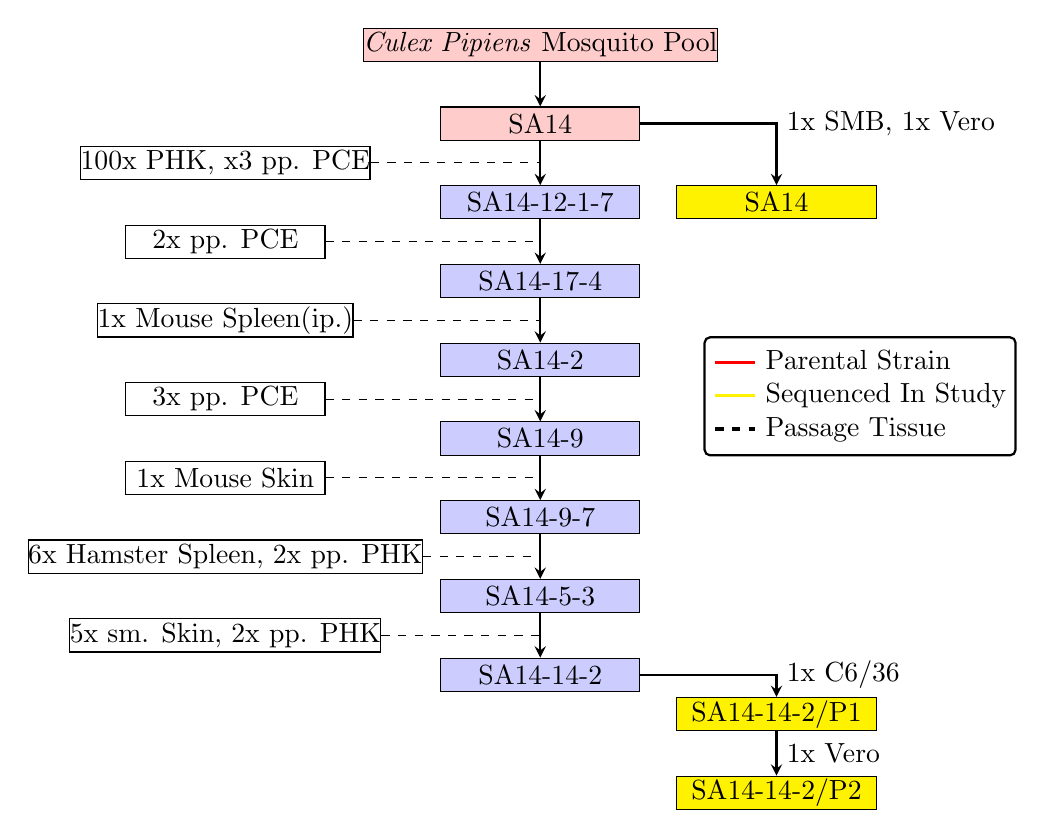
\begin{tikzpicture}[auto]

%\draw[help lines,step=.5] (0,0) grid (12,12);

	%Nodes for each of the strains mentioned by Yu 2010
	\node[parent](Mosquito) at (6,12) {\emph{Culex Pipiens} Mosquito Pool};
	\node[parent, below of=Mosquito](SA14){SA14};
	\node[intermediate, below of=SA14](SA14-12-1-7){SA14-12-1-7};
	\node[intermediate, below of=SA14-12-1-7](SA14-17-4){SA14-17-4};
	\node[intermediate, below of=SA14-17-4](SA14-2){SA14-2};
	\node[intermediate, below of=SA14-2](SA14-9){SA14-9};
	\node[intermediate, below of=SA14-9](SA14-9-7){SA14-9-7};
	\node[intermediate, below of=SA14-9-7](SA14-5-3){SA14-5-3};
	\node[intermediate, below of=SA14-5-3](SA14-14-2){SA14-14-2};
%	\node[intermediate, below of=SA14-14-2](SA14-14-2-PDK){SA14-14-2 PDK};
	
	%Nodes for each of the three strains considered in the study.
	\node[studied](TYF2350) at ([xshift=3cm,yshift=-1cm]SA14) {SA14};
	\node[studied](TYF1454)at ([xshift=3cm,yshift=-0.5cm]SA14-14-2){SA14-14-2/P1};
	\node[studied, below of=TYF1454](TYF1910){SA14-14-2/P2};	

	%Arrows connecting the three strains considered in the study.
	\path[arrow] (SA14-14-2) -| node {1x C6/36}(TYF1454);
	\path[arrow] (TYF1454) -- node {1x Vero} (TYF1910);
	\path[arrow] (SA14) -| node{1x SMB, 1x Vero} (TYF2350);
	
	%Arrow connecting Paths
	\path[arrow] (Mosquito) -- coordinate[midway](M1) (SA14);
	\path[arrow] (SA14) -- coordinate[midway](M2) (SA14-12-1-7);
	\path[arrow] (SA14-12-1-7) -- coordinate[midway](M3) (SA14-17-4);
	\path[arrow] (SA14-17-4) -- coordinate[midway](M4) (SA14-2);
	\path[arrow] (SA14-2) -- coordinate[midway](M5) (SA14-9);
	\path[arrow] (SA14-9) -- coordinate[midway](M6) (SA14-9-7);
	\path[arrow] (SA14-9-7) -- coordinate[midway](M7) (SA14-5-3);
	\path[arrow] (SA14-5-3) -- coordinate[midway](M8) (SA14-14-2);
%	\path[arrow] (SA14-14-2) -- coordinate[midway](M9) (SA14-14-2-PDK);

	%Nodes for the passage information
%	\node[information](Mosquito_pass) at ([xshift=-4cm]M1) {11x mb.};
	\node[information](SA14_pass) at ([xshift=-4cm]M2) {100x PHK, x3 pp. PCE};
	\node[information](SA14-12-1-7_pass) at ([xshift=-4cm]M3) {2x pp. PCE};
	\node[information](SA14-17-4_pass) at ([xshift=-4cm]M4) {1x Mouse Spleen(ip.)};
	\node[information](SA14-2_pass) at ([xshift=-4cm]M5) {3x pp. PCE};
	\node[information](SA14-9_pass) at ([xshift=-4cm]M6) {1x Mouse Skin};
	\node[information](SA14-9-7_pass) at ([xshift=-4cm]M7) {6x Hamster Spleen, 2x pp. PHK};
	\node[information](SA14-5-3_pass) at ([xshift=-4cm]M8) {5x sm. Skin, 2x pp. PHK};
%	\node[information](SA14-14-2_pass) at ([xshift=-4cm]M9) {9x PDK};

	%Paths connecting passage information nodes with center of arrows.
%	\path[line,dashed] (Mosquito_pass) -- (M1);	
	\path[line,dashed] (SA14_pass) -- (M2);	
	\path[line,dashed] (SA14-12-1-7_pass) -- (M3);	
	\path[line,dashed] (SA14-17-4_pass) -- (M4);
	\path[line,dashed] (SA14-2_pass) -- (M5);	
	\path[line,dashed] (SA14-9_pass) -- (M6);	
	\path[line,dashed] (SA14-9-7_pass) -- (M7);	
	\path[line,dashed] (SA14-5-3_pass) -- (M8);	
%	\path[line,dashed] (SA14-14-2_pass) -- (M9);	

					
	\node[draw=black,thick,rounded corners=2pt,below left=2mm] at (12.25,8.5) {%
		\begin{tabular}{@{}r@{ }l@{}}
		%	\raisebox{2pt}{\tikz{\draw[gray, very thick, dashed] (0,0) -- (5mm,0);}}&National Origin\\
		\raisebox{2pt}{\tikz{\draw[red, very thick] (0,0) -- (5mm,0);}}&Parental Strain\\
		\raisebox{2pt}{\tikz{\draw[yellow, very thick] (0,0) -- (5mm,0);}}&Sequenced In Study\\
		\raisebox{2pt}{\tikz{\draw[black,dashed, very thick] (0,0) -- (5mm,0);}}&Passage Tissue\\
		\end{tabular}};
\end{tikzpicture}
	\caption[Derivation of JEV Vaccine, showing the passage history of newly analyzed strains.]{Derivation of \gls{jev} Vaccine, showing the passage history of newly analyzed strains. PCE = Primary Chick Embryo, PHK = Primary Hamster Kidney, pp. = Plaque Pick, SMB = Suckling Mouse Brain.}
\label{JEV_tree}
\end{figure}
\clearpage

\begin{figure}[p]
	\centering
	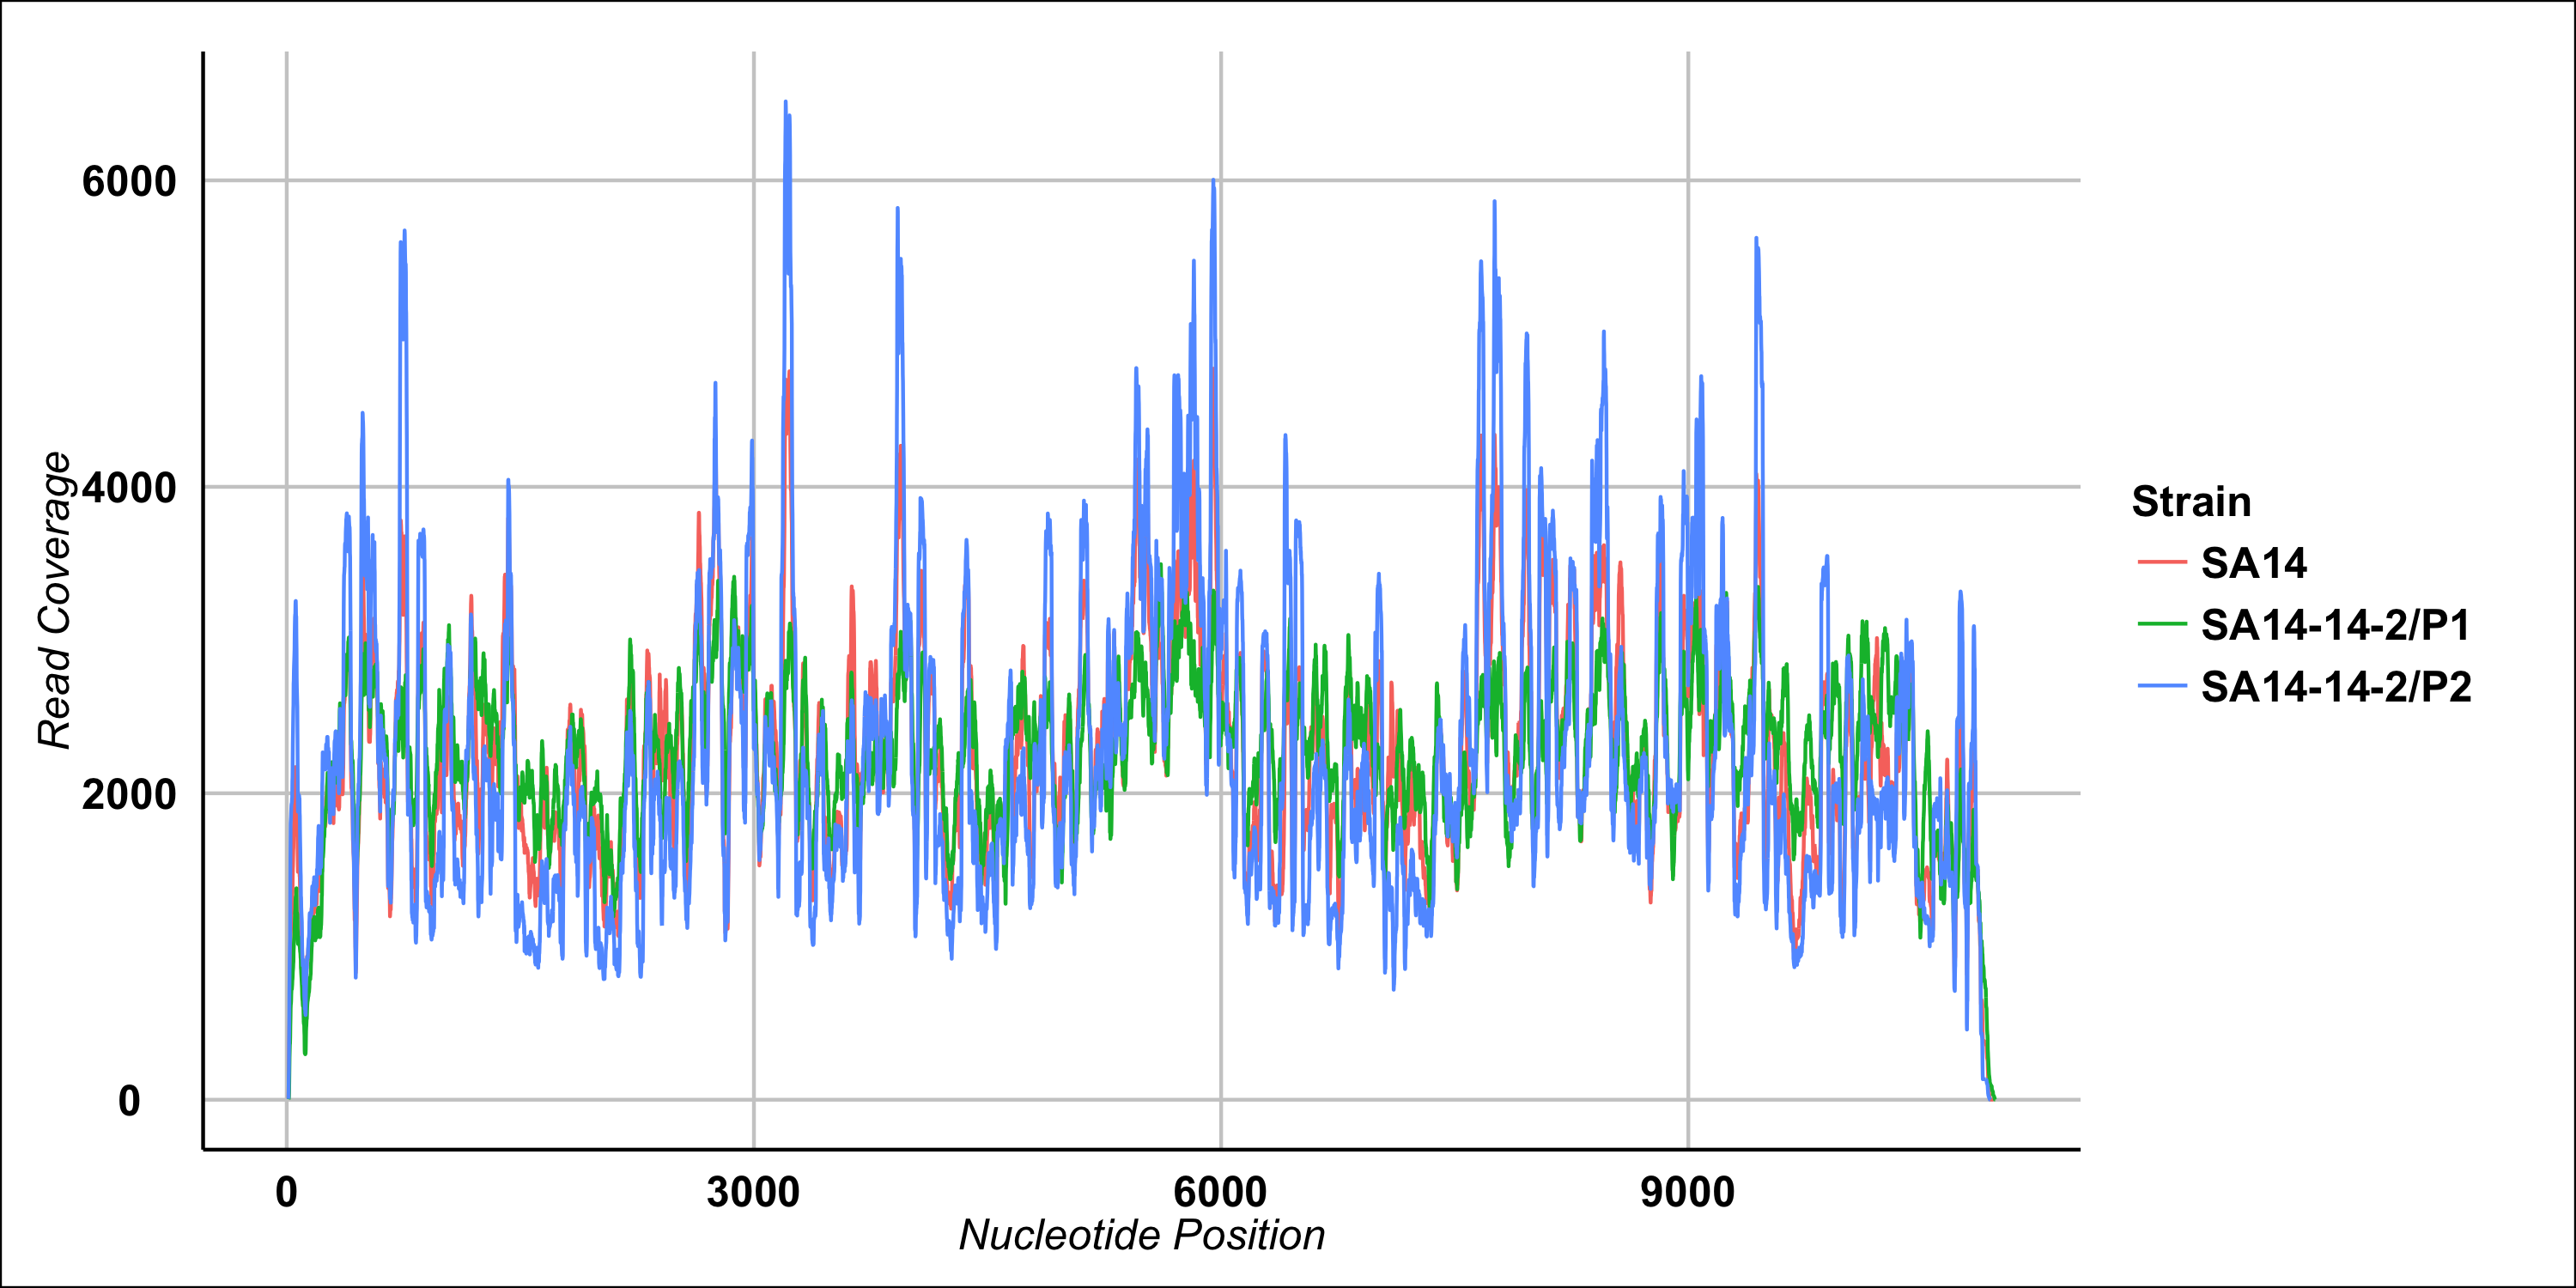
\includegraphics[width = \columnwidth]{../FIGURES/Chapter_JEV_FIGURE/coverage_plot_FIGURE/coverage_plot.png}
	\caption{Read coverage along the length of genomes, for each virus analyzed in the study.}
\label{JEV_coverage}
\end{figure}
\clearpage

\begin{figure}[p]
	\centering
	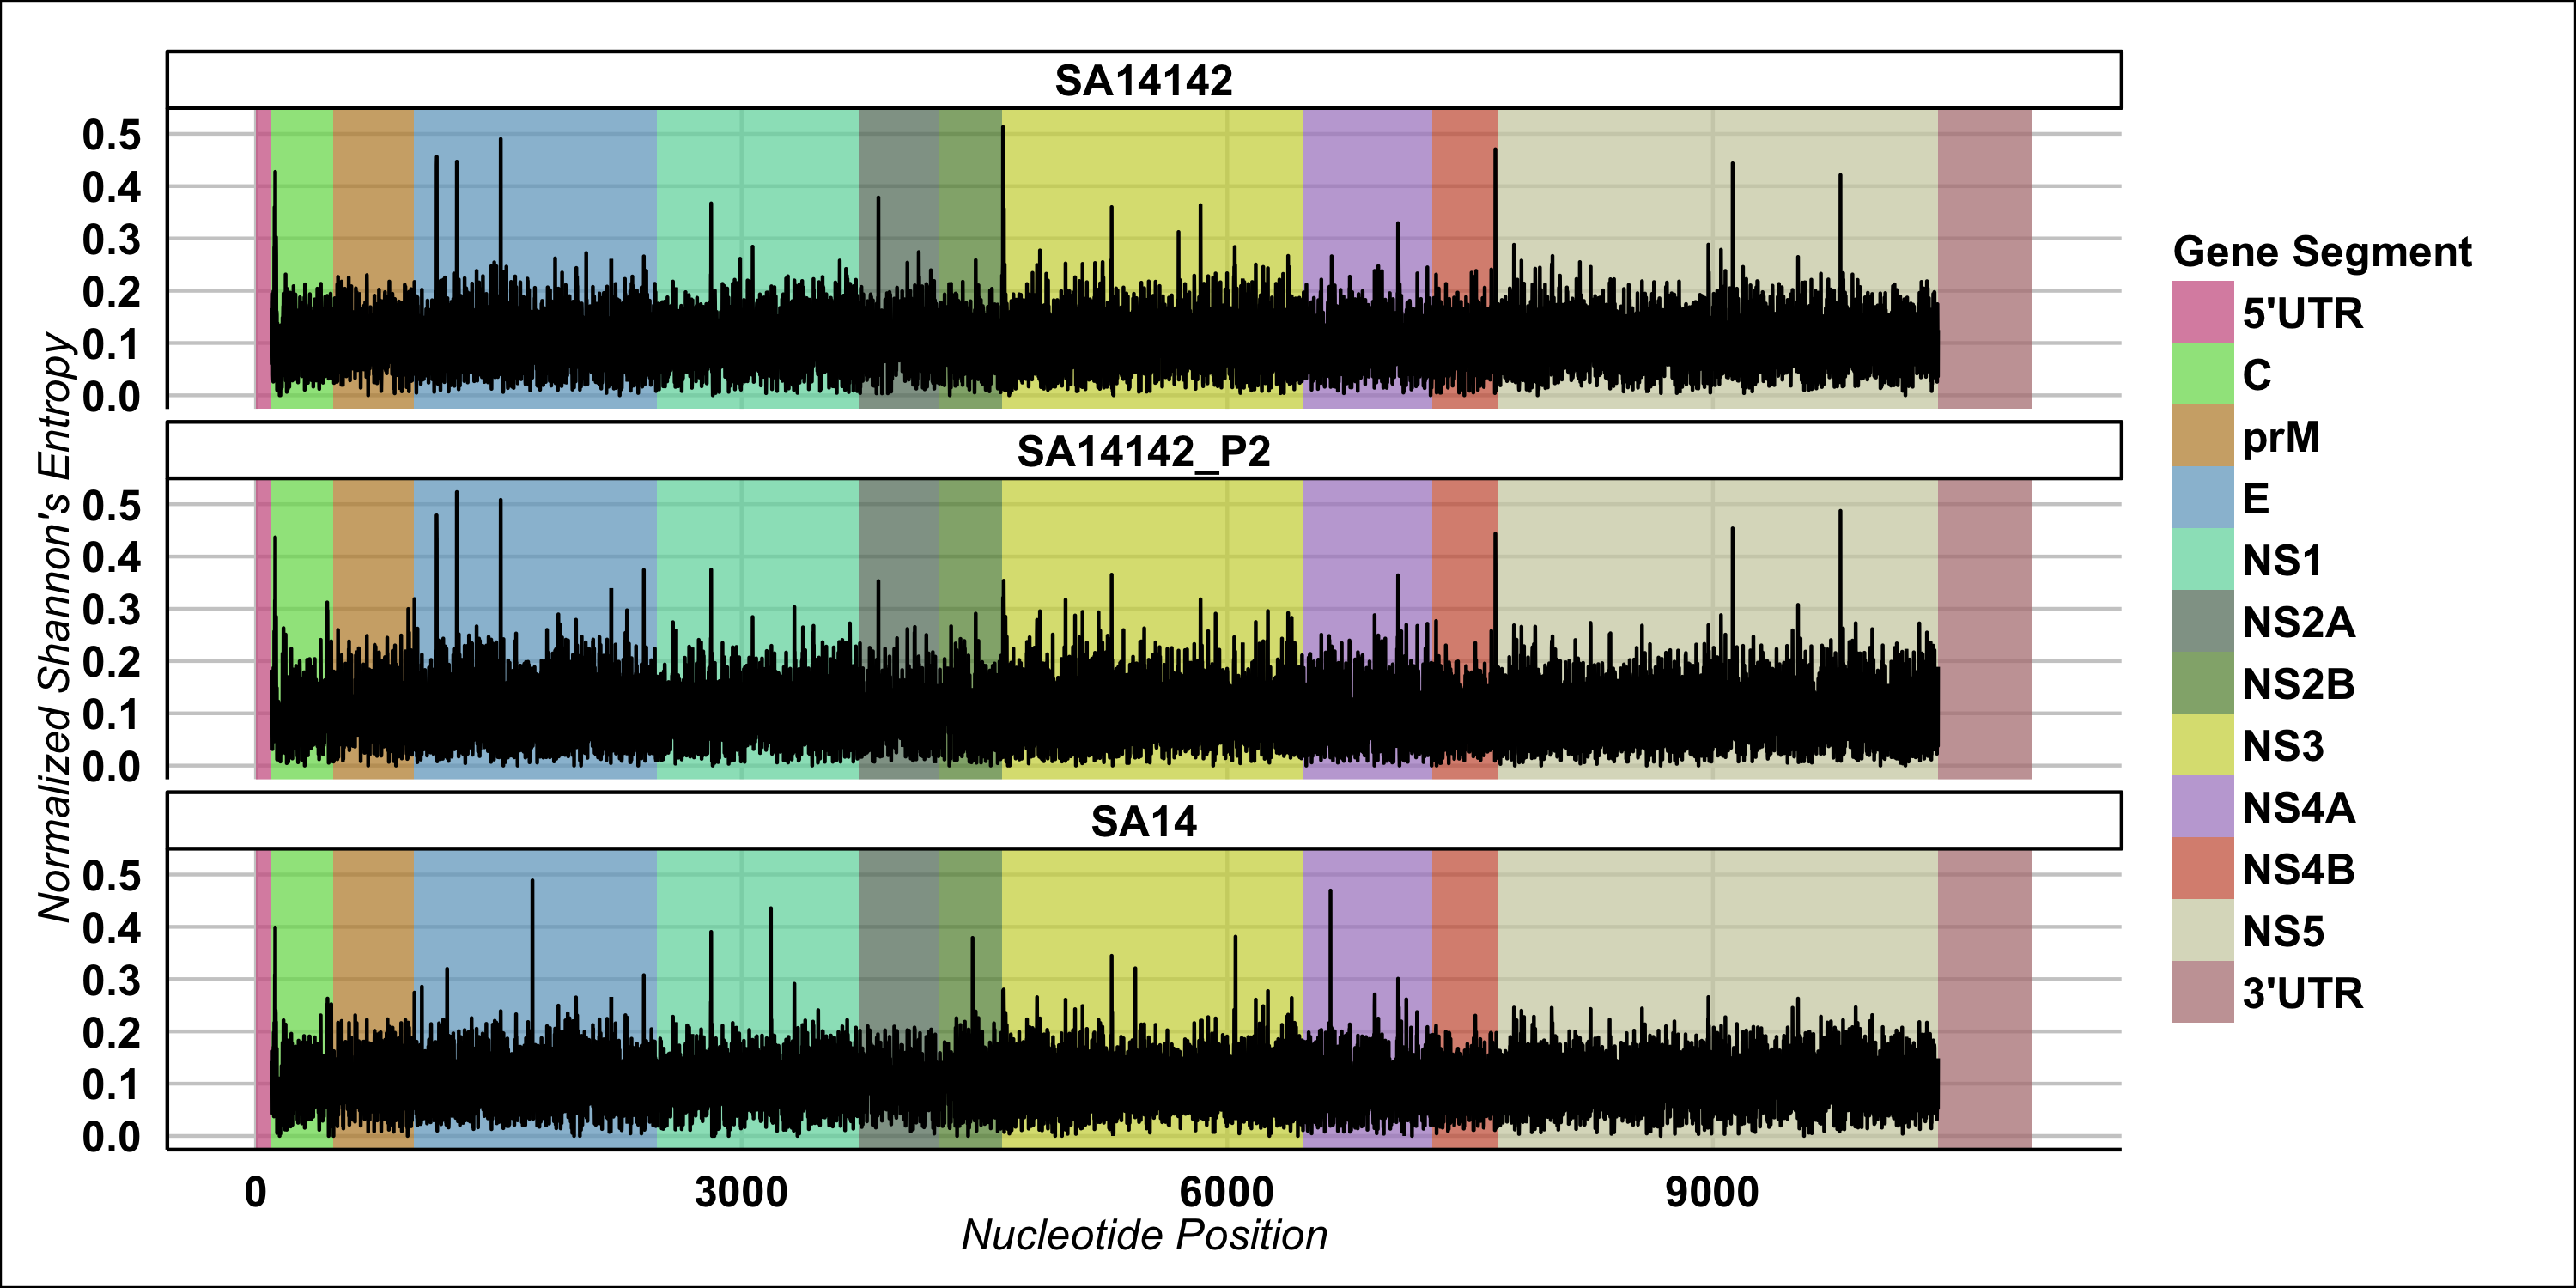
\includegraphics[width = \columnwidth]{../FIGURES/Chapter_JEV_FIGURE/entropy_sitewise_FIGURE/entropy_sitewise_FIGURE.png}
	\caption[Sitewise diversity estimation, measured by normalized Shannon's entropy, for each strain considered in the study.]{Sitewise diversity estimation, measured by \gls{nse}, for each strain considered in the study. Diversity was estimated at each nucleotide position recovered in the read alignment for the \gls{jev} strains SA14, SA14-14-2/P1, and SA14-14-2/P2.}
	\label{JEV_entropy_whole}
\end{figure}
\clearpage

\begin{figure}[p]
	\centering
	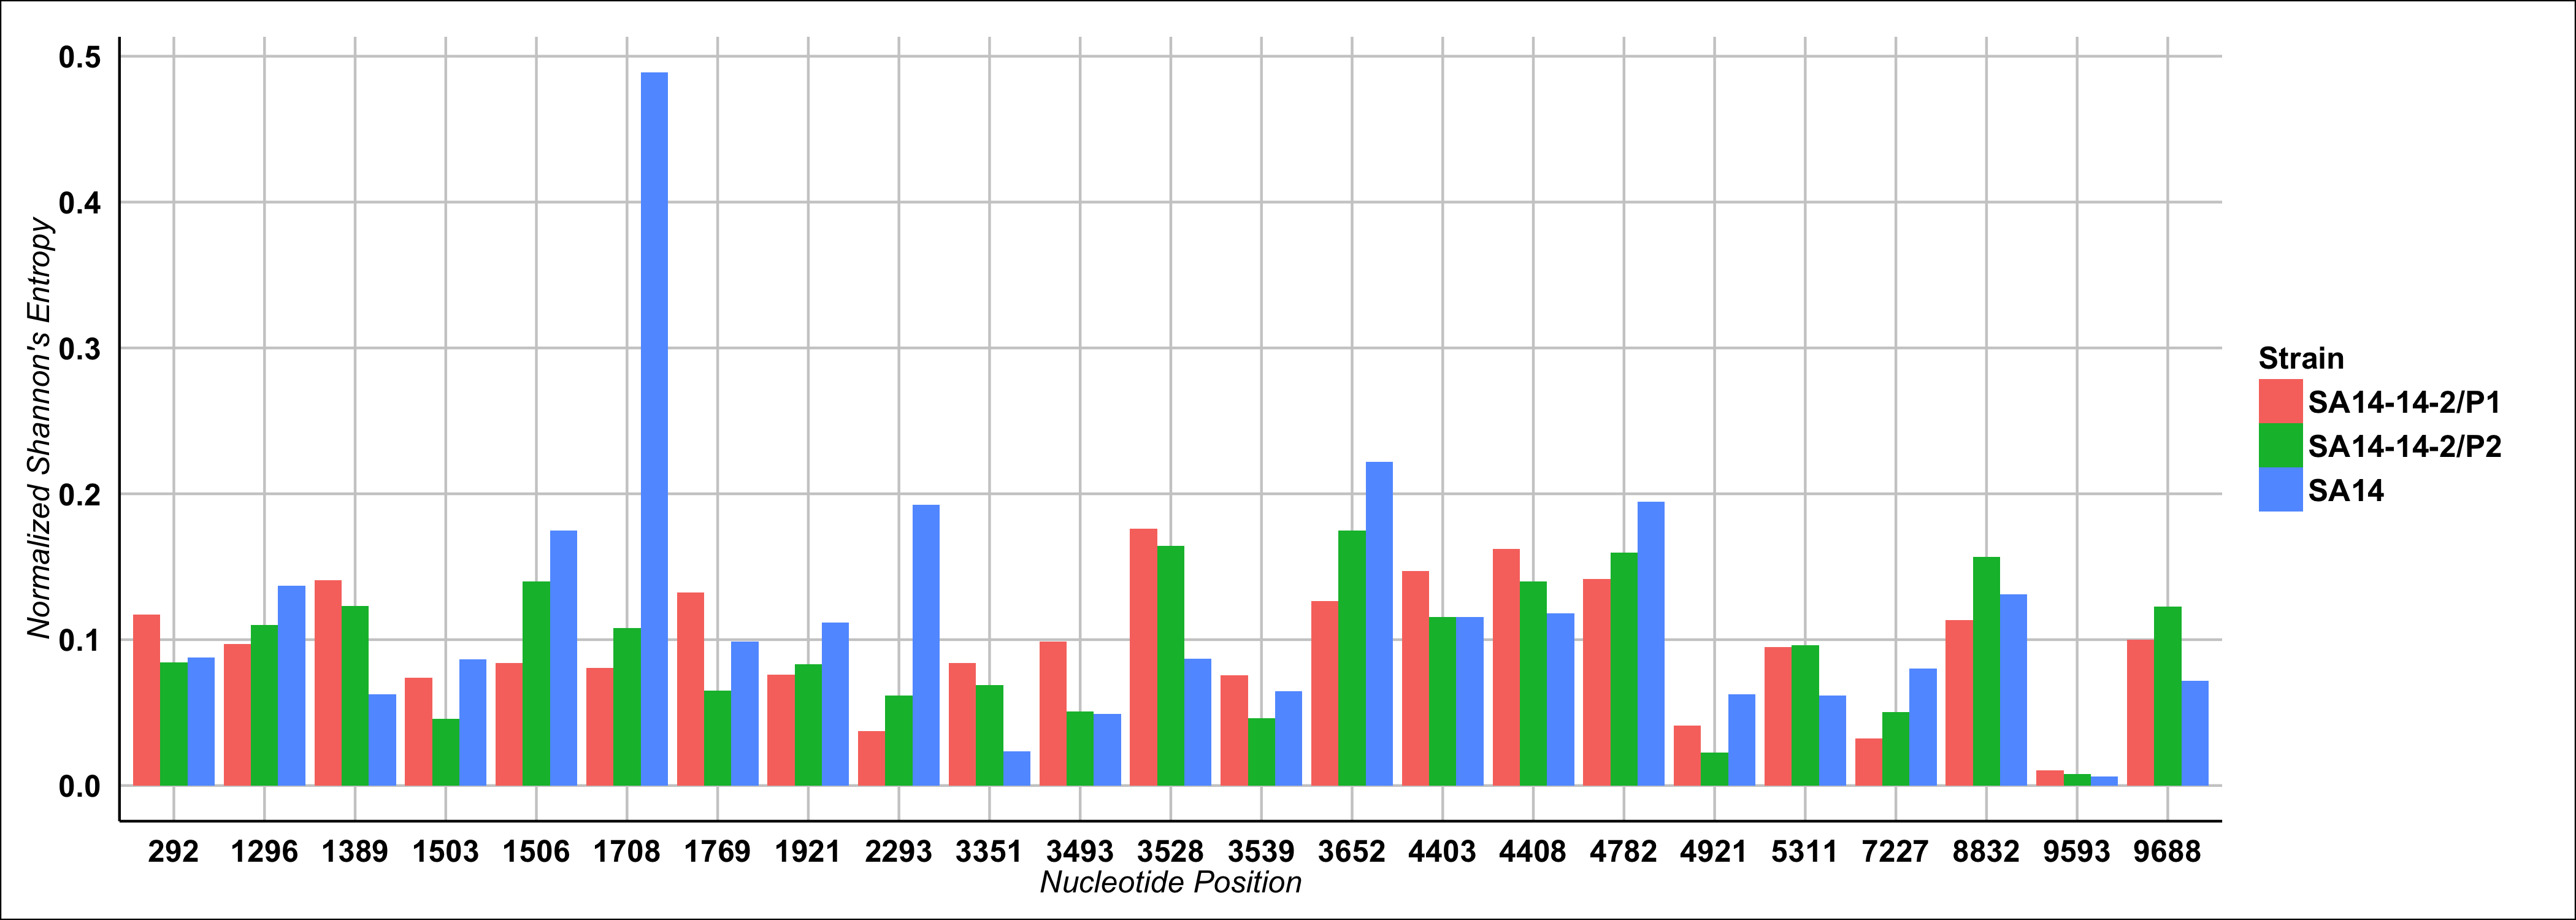
\includegraphics[width = \columnwidth]{../FIGURES/Chapter_JEV_FIGURE/AA_vaccineset_FIGURE/AA_vaccineset_FIGURE.png}
	\caption[Summary of diversity, measured by normalized Shannon’s entropy, for each nucleotide position containing an amino acid substitution between the newly sequenced wild-type strain SA14 and vaccine strains SA14-14-2/P1 or SA14-14-2/P2.]{Summary of diversity, measured by \gls{nse}, for each nucleotide position containing an amino acid substitution between the newly sequenced wild-type strain SA14 and vaccine strains SA14-14-2/P1 or SA14-14-2/P2.}
	\label{JEV_barplot}
\end{figure}
\clearpage

\begin{figure}[p]
	\centering
	
\includegraphics[width = \columnwidth]{../FIGURES/Chapter_JEV_FIGURE/scatter_RMSD_FIGURE/genewise_scatter_FIGURE.png}
	\caption[A plot of normalized Shannon’s entropy versus RMSD relative to the wild-type parental strain SA14, for each nucleotide position recovered in the three JEV strains.]{A plot of normalized Shannon’s entropy versus \gls{rmsd} relative to the wild-type parental strain SA14, for each nucleotide position recovered in the three \gls{jev} strains. SA14 is shown to control, and are clustered at implied zero distance and relatively higher diversity than the vaccines. Colored points represent the nucleotide positions that with amino acid substitutions in the vaccine strains relative to SA14. Clustering of points these at high genetic distance from the parental strain is shown, and is evidence for selection of the vaccine genotype.}
	\label{JEV_scatter_RMSD}
\end{figure}
\clearpage

\begin{figure}[p]
	\centering
	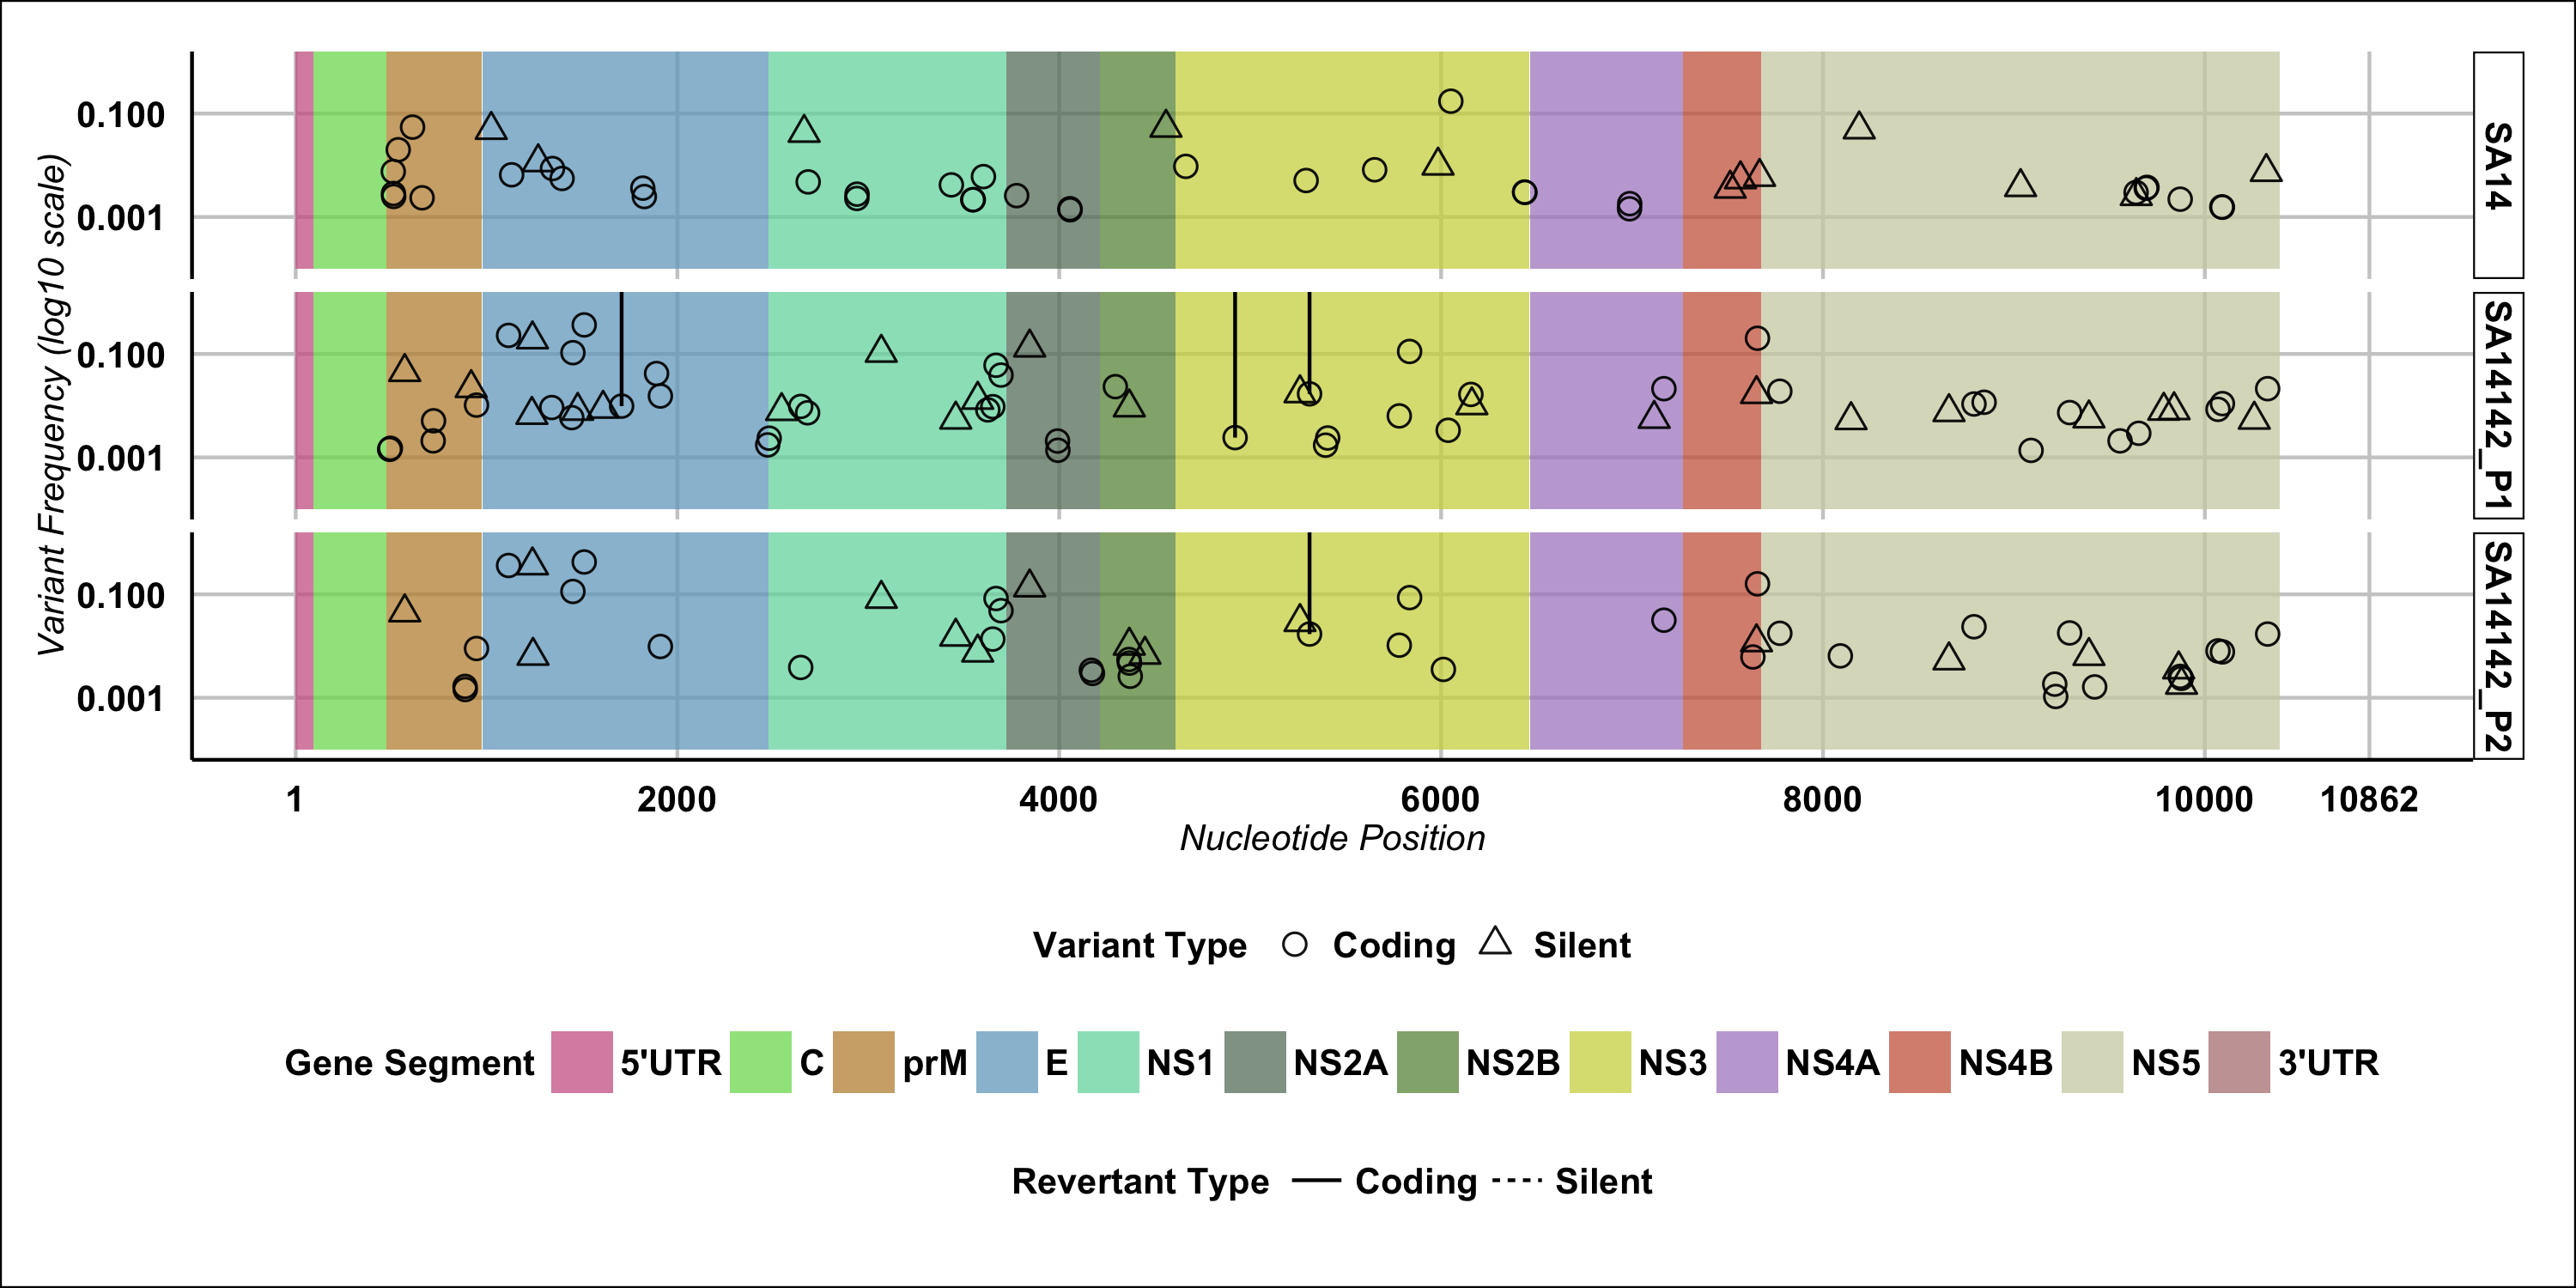
\includegraphics[width = \columnwidth]{../FIGURES/Chapter_JEV_FIGURE/variants_vphaser_FIGURE/variants_vphaser_FIGURE.png}
	\caption[A plot of the frequency of each SNV recovered from the JEV strains studied by a probabilistic model in V-Phaser v. 2.0, in order of nucleotide position.]{A plot of the frequency of each \gls{snv} recovered from the \gls{jev} strains studied by a probabilistic model in V-Phaser v. 2.0, in order of nucleotide position. \glspl{snv} are classified as either silent(triangle glyph) or coding (circle glyph) relative to the consensus of the strain considered; as well the \glspl{snv} are classified for reversion to the wild-type genotype identified by vertical line segments.}
	\label{JEV_vphaser}
\end{figure}
\clearpage

\begin{figure}[p]
	\centering
	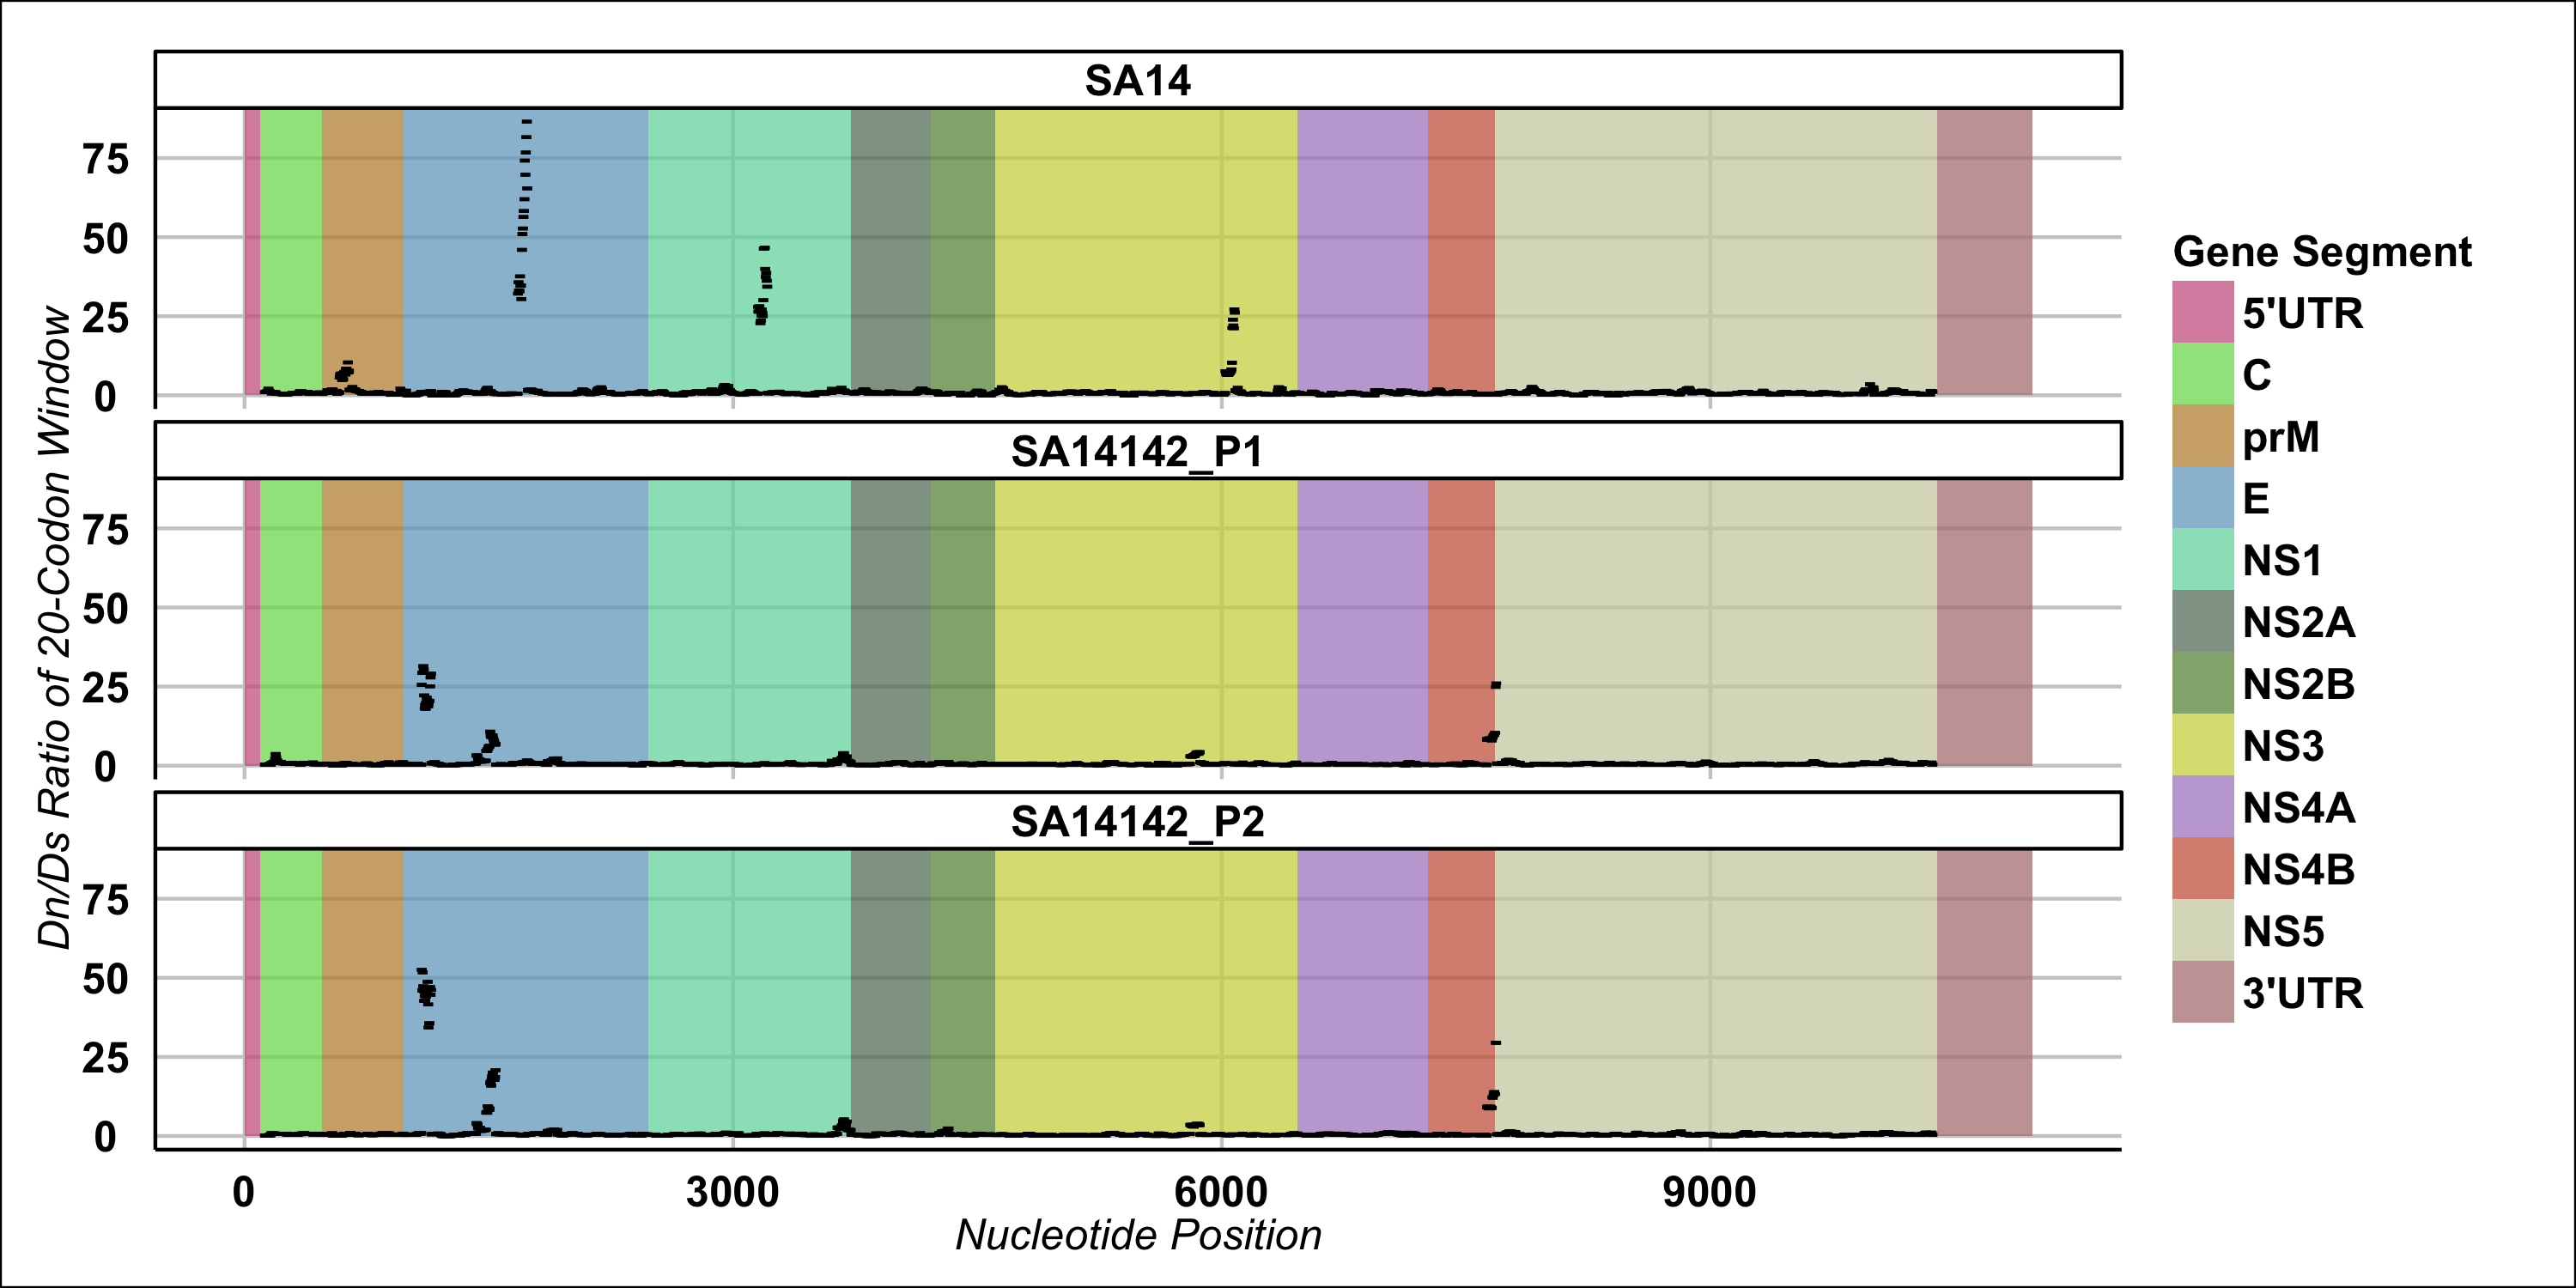
\includegraphics[width = \columnwidth]{../FIGURES/Chapter_JEV_FIGURE/DNDS_20codon_FIGURE/DNDS_20.png}
	\caption[20-codon sliding window analysis of $dN/dS$, along the open reading frames of JEV strains SA14. SA14-14-2/P1, and SA14-14-2/P2.]{20-codon sliding window analysis of $dN/dS$, along the open reading frames of JEV strains SA14. SA14-14-2/P1, and SA14-14-2/P2. Broadly, ratios along the length of the JEV genomes are low, indicative of purifying selection and a stable population. A small number of regions are influenced by apparent positive selection,
		in which $dN/dS$ exceeds 1.000.}
	\label{JEV_20codon}
\end{figure}
\clearpage

